\documentclass[a4paper,onecolumn,12pt]{report} 

\usepackage{a4wide}
\usepackage[printonlyused]{acronym}
\usepackage{amsmath}
\usepackage{amssymb}
\usepackage{array}
\usepackage{boxedminipage}
\usepackage{cite}
\usepackage{color}
\usepackage{fancyvrb}
\usepackage[draft]{fixme}
\usepackage{forloop}
\usepackage[pdftex]{graphicx}
\usepackage{helvet}
\usepackage[colorlinks,linkcolor=black,urlcolor=blue]{hyperref}
\usepackage{ifthen}
\usepackage{listings}
\usepackage{longtable}
\usepackage{subfig}
\usepackage{tikz}
\usepackage{verbatim}
\usepackage{xspace}

\newboolean{Solutions} \setboolean{Solutions}{true}

\renewcommand{\chaptername}{Lab}
\newcommand{\stress}[1]{\emph{\textbf{#1}}} 
\newcommand{\command}[1]{\texttt{#1}\newline} 
\newcommand{\incommand}[1]{\texttt{#1}}
\newcommand{\file}[2]{\texttt{/mnt/L\arabic{chapter}-\arabic{Exercisecount}-\stepcounter{questioncount}\arabic{questioncount}\addtocounter{questioncount}{-1}.#1}} 
\newcommand{\curfile}[2]{\texttt{/mnt/L\arabic{chapter}-\arabic{Exercisecount}-\stepcounter{questioncount}\arabic{questioncount}\addtocounter{questioncount}{-1}.#1}} 
\newcommand{\remark}{
\includegraphics{images/remark.pdf}}
\newcommand{\report}{ 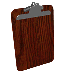
\includegraphics{images/report.pdf}}

\newcommand{\result}[1]{
\begin{verbatim}
	#1 
\end{verbatim}
} 
\newcommand{\prompt}[1]{#1:\textasciitilde\#}


%%%%%%%%%%%%%%%%%%%%%%%%%%%%%%%%%%%%%%
% exercise environment
%%%%%%%%%%%%%%%%%%%%%%%%%%%%%%%%%%%%%%

\newcounter{Exercisecount}[chapter]
\setcounter{Exercisecount}{0}
\newenvironment{exercise}[1]
{% This is the begin code
\refstepcounter{Exercisecount} {\textbf {Exercise \arabic{Exercisecount}}}: #1
}
{% This is the end code
 }

%%%%%%%%%%%%%%%%%%%%%%%%%%%%%%%%%%%%%%
% question counter environment
%%%%%%%%%%%%%%%%%%%%%%%%%%%%%%%%%%%%%%
\newcounter{questioncount}[Exercisecount]
\setcounter{questioncount}{0}

\newcommand{\answerlabel}{L\arabic{chapter}-\arabic{Exercisecount}-\arabic{questioncount}}

\newcommand{\answer}{
\begin{tikzpicture}
 
\node [fill=shade,rounded corners=5pt]
{
\refstepcounter{questioncount}
\color{white}{\textbf{\answerlabel}}
};
\end{tikzpicture}
}

\newcommand{\includeanswer}{\input{solutions/\answerlabel.tex}}


%%%%%%%%%%%%%%%%%%%%%%%%%%%%%%%%%%%%%%
% verbatim solution environment
%%%%%%%%%%%%%%%%%%%%%%%%%%%%%%%%%%%%%%
%\newcounter{linescounter}
%\newenvironment{esolution}[1]
%{
%\answer
%\ifthenelse{\boolean{Solutions}}
%{
%\color{blue}
%
%\hrulefill
%
%\includeanswer
%
%}
%{\setlength{\extrarowheight}{0.75cm} 
%
%\forloop{linescounter}{0}{\value{linescounter}<#1}{\quad\newline\vspace{12pt} \dotfill\newline}
%\comment
%}
%}

\newenvironment{esolution}
{
\answer
\ifthenelse{\boolean{Solutions}}
{
\color{blue}

\hrulefill

\includeanswer

}
{\setlength{\extrarowheight}{0.75cm} 
\quad\newline\vspace{12pt} \dotfill\newline
\comment
}
}
{
\ifthenelse{\boolean{Solutions}}
{

\hrulefill

}
{\endcomment}
}


\DefineVerbatimEnvironment{Verbatim}{Verbatim}
{formatcom=\color{blue},fontfamily=courier,fontseries=b,frame=lines,numbers=left}





%%%%%%%%%%%%%%%%%%%%%%%%%%%%%%%%%%%%%%
% shortcuts
%%%%%%%%%%%%%%%%%%%%%%%%%%%%%%%%%%%%%%
\newcommand{\wifi}{IEEE 802.11\xspace}

%%%%%%%%%%%%%%%%%%%%%%%%%%%%%%%%%%%%%%
% fonts
%%%%%%%%%%%%%%%%%%%%%%%%%%%%%%%%%%%%%%
\renewcommand{\rmdefault}{phv}
\renewcommand{\sfdefault}{phv}

%%%%%%%%%%%%%%%%%%%%%%%%%%%%%%%%%%%%%%
% colors
%%%%%%%%%%%%%%%%%%%%%%%%%%%%%%%%%%%%%%
\definecolor{shade}{HTML}{3877A9}	%light blue shade
\setlength{\parskip}{10pt plus 1pt minus 1pt}

\lstset{ %
basicstyle=\footnotesize,       % the size of the fonts that are used for the code
numbers=left,                   % where to put the line-numbers
numberstyle=\footnotesize,      % the size of the fonts that are used for the line-numbers
stepnumber=2,                   % the step between two line-numbers. If it's 1, each line 
                                % will be numbered
numbersep=5pt,                  % how far the line-numbers are from the code
backgroundcolor=\color{white},  % choose the background color. You must add \usepackage{color}
showspaces=false,               % show spaces adding particular underscores
showstringspaces=false,         % underline spaces within strings
showtabs=false,                 % show tabs within strings adding particular underscores
frame=single,                   % adds a frame around the code
tabsize=2,                      % sets default tabsize to 2 spaces
captionpos=b,                   % sets the caption-position to bottom
breaklines=true,                % sets automatic line breaking
breakatwhitespace=false,        % sets if automatic breaks should only happen at whitespace
title=\lstname,                 % show the filename of files included with \lstinputlisting;
                                % also try caption instead of title
escapeinside={\%*}{*)},         % if you want to add a comment within your code
morekeywords={*,...}            % if you want to add more keywords to the set
}
%If the variable below is set to 'false', dotted lines are generated where answers are expected.
%If it is set to 'true', LaTeX will search for the files specified in the document in the 'solutions' folder and include their contents where the answers are expected.
\setboolean{Solutions}{true}
%%%%%%%%%%%%%%%%%%%%%%%%%%%%%%%%%%%%%%%%%%%%%%%%
%        Fill in your names                    %
%%%%%%%%%%%%%%%%%%%%%%%%%%%%%%%%%%%%%%%%%%%%%%%%
%\author{Name 1 \and Name 2}  
%%%%%%%%%%%%%%%%%%%%%%%%%%%%%%%%%%%%%%%%%%%%%%%%
\author{Thomas Hendriks \and Jakob Struye}

\title{Advanced Networking Lab}

\begin{document}


%\frontmatter
\maketitle

%\mainmatter
%\input{intro.tex}
%!TEX root = labo.tex
\setcounter{chapter}{0}
\chapter{Basic Configurations}

The goal of the first lab is to make you acquainted with the hardware and software needed to perform the tasks in other modules. Furthermore we will have a look at the various sniffing possibilities in wireless networks.

\section{Device Exploration}

Have a closer look a the devices used for this course. 

\begin{exercise}{Getting to know the interfaces}
	\begin{enumerate}
		\item Log in on \ac{wmn}1. \newline
		\command{ssh root@wmn1}
		\item When asked to give a name, enter
		\command{AP}
		\item Get a list of all available interfaces. \newline
		\command{\prompt{\acs{ap}} ifconfig -a}
		\item List the interfaces and their \ac{mac} addresses.\newline		\begin{esolution}
		\end{esolution}
		\item A \ac{mac} address is unique per card, but also carries a generic part, identifying the vendor of a card. List the prefixes and find out the vendors (name) of all different interfaces found in the node.\\
		\remark Google is your friend!\newline		
		\begin{esolution}
		\end{esolution}
	\end{enumerate}
	
\end{exercise}

\section{Access Point Setup}

\begin{figure}[h]
	\begin{center}
		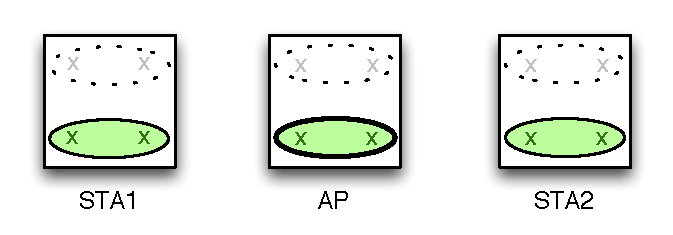
\includegraphics[width=0.8\textwidth]{images/snif1.pdf} 
		\caption{The basic infrastructure setup}
		\label{fig:basic-infra}  
	\end{center}
\end{figure}

The goal is to create a basic infrastructure setup as can be found at home. The setup consists of one \ac{ap} and two connected stations as shown in figure \ref{fig:basic-infra}. In this case, two laptops are connected to the same \ac{ap} and can communicate to each other. We will not consider any communication to the outside world.

\subsection{\ac{ap} Configuration}
To set up this basic infrastructure network, start by configuring the \ac{ap}.

\begin{exercise}{Set up an \ac{ap}}
\begin{enumerate}
	\item Check the wireless parameters of wlan1:\newline
	\command{\prompt{\acs{ap}} iwconfig wlan1}\newline
	This should give you some output like
\begin{verbatim}
wlan1     IEEE 802.11abgn  ESSID:off/any  
          Mode:Managed  Access Point: Not-Associated   Tx-Power=0 dBm   
          RTS thr:off   Fragment thr:off
          Encryption key:off
          Power Management:off
\end{verbatim}

\remark Remark that we did not configure the interface yet!

Give an explanation for all available parameters which are displayed using \incommand{iwconfig} (hint: man pages).\newline
\begin{esolution}
\end{esolution}


\item Configure the wlan1 interface using your assigned channel and the \ac{essid}:\newline
\begin{lstlisting}
interface=wlan
driver=nl80211
logger_syslog=-1
logger_syslog_level=2
logger_stdout=-1
logger_stdout_level=2
debug=4
hw_mode=a
channel=x
macaddr_acl=0
auth_algs=3
eapol_key_index_workaround=0
eap_server=0
wpa=0
ssid=wmn-gid-A
\end{lstlisting}

This file can be found on the devices as \texttt{hostapd.conf}. Edit it to change the channel number, interface name and \ac{essid}, and then perform the following:\newline
\command{\prompt{\acs{ap}} hostapd -B hostapd.conf}

\incommand{\prompt{\acs{ap}} iwconfig} should now return something like: 
\begin{verbatim}
wlan1     IEEE 802.11abgn  Mode:Master  Tx-Power=20 dBm   
          RTS thr:off   Fragment thr:off
          Power Management:off
\end{verbatim}

\end{enumerate}
\end{exercise}

\subsection{Station Configuration}

\begin{exercise}{Configuring the wireless stations}
	
We will now configure \emph{both} stations  and verify they get associated with the \ac{ap} you just created. Make sure to repeat the commands to configure the second station.

\begin{enumerate}
	\item Bring up the interface: \newline
	\command{\prompt{\acs{sta}1} ifconfig wlan1 up}
	\item Configure the interface to connect to our \ac{ap}: \newline
	\command{\prompt{\acs{sta}1} iw dev wlan1 connect \ac{wmn}-\acs{gid}-A}
	\item Do the same on \ac{sta}2.



\remark When you run \incommand{iwconfig}, the \incommand{Access Point} parameter should show the \ac{mac} address of the \ac{ap} and show identical frequencies and \acp{essid} on both stations. 
\begin{verbatim}
wlan1     IEEE 802.11abgn  ESSID:"wmn-0-A"  
          Mode:Managed  Frequency:5.24 GHz  Access Point: 00:00:11:22:33:44   
          Bit Rate=1 Mb/s   Tx-Power=5 dBm   
          RTS thr:off   Fragment thr:off
          Encryption key:off
          Power Management:off
          Link Quality=12/70  Signal level=-164 dBm  
          Rx invalid nwid:0  Rx invalid crypt:0  Rx invalid frag:0
          Tx excessive retries:0  Invalid misc:4   Missed beacon:0
\end{verbatim}
	\item What parameters are different in your output compared to the output above?\newline
	\begin{esolution}
	\end{esolution}
\end{enumerate}
\end{exercise}

If the output for both stations confirms the association between the two wireless stations and the \ac{ap}, the actual L2 connection between these three devices is up and running. To verify the connection, we will configure IP addresses on the stations and have them communicate.

\begin{exercise}{Verifying the basic setup}\label{ex:pingtest}
	
	\begin{enumerate}
		\item Configure the IP address of \ac{sta}1 and \ac{sta}2:\newline
		\command{\prompt{\ac{sta}1} ip addr add fc00::\acs{gid}::1/64 dev wlan1}
		\command{\prompt{\ac{sta}2} ip addr add fc00:\acs{gid}::2/64 dev wlan1}
		\item Start a ping session from \ac{sta}1 to \ac{sta}2. Give the minimum, maximum and average \ac{rtt}:\newline
		\command{\prompt{\ac{sta}1} ping6 -c 30 fc00:\acs{gid}::2}
		\begin{esolution}
		\end{esolution}
		\item Perform a ping between the same devices as before, but this time, use the wired IP addresses. Again write down the same values.\newline
		\begin{esolution}
		\end{esolution}
	\end{enumerate}
\end{exercise}

\remark Remark that we did not (yet) enable L3 capabilities at the \ac{ap}.


\section{Wireless Sniffing}

Using the basic network we constructed in the previous section, we will go through the various sniffing modes available in wireless networks. The main difference between wired and wireless networks is obviously the fact that the transmission medium (radio waves vs. cable) is shared amongst all wireless users. Therefore, sniffing the network offers a lot more opportunities in wireless systems.
\begin{figure}
	\begin{center}
		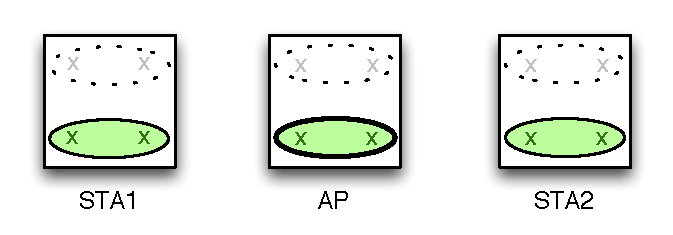
\includegraphics[width=0.5\textwidth]{images/snif1.pdf} 
		\caption{Wireless packet capture setup} 
		\label{fig:snif1} 
	\end{center}
\end{figure}


The first setup is shown in figure \ref{fig:snif1} and corresponds to the basic setup we created in the previous section. 



\begin{exercise}{First scan}\label{ex:firstScan}
\begin{enumerate}
	\item Make sure the \ac{nd} cache of both \acp{sta} is cleared.\label{ex:1-1}\newline
	\command{\prompt{\ac{sta}2} ip neigh flush dev wlan1}
	\command{\prompt{\ac{sta}1} ip neigh flush dev wlan1}
	\remark You can always check the state of the cache using \command{ip neigh show}
	\item On the \ac{ap} and on both \acp{sta}, start a packet capture using \incommand{tcpdump} and save it to \file{snif-location.pcap}. \newline
	\remark This is the time to make sure that you have a remote location mounted with \verb!sshfs! in /mnt!\newline\newline
	\command{\prompt{\acs{ap}} tcpdump -i wlan1 -w \file{\acs{ap}.pcap}}
	\command{\prompt{\acs{sta}1} tcpdump -i wlan1 -w \file{\acs{sta}1.pcap}}
	\command{\prompt{\acs{sta}2} tcpdump -i wlan1 -w \file{\acs{sta}2.pcap}}
	\item Start a ping session from \ac{sta}1 to \ac{sta}2. Limit the ping to only two requests. \label{ex:1-3}\newline
	\command{\prompt{\ac{sta}1} ping6 -c 2 fc00:\acs{gid}::2} 
	\item Which type of packets can be seen in the \acs{ap} trace file? You can open the trace file with wireshark on the remote computer.\newline
	\begin{esolution}
	\end{esolution}
	\item Now, take a closer look at the \ac{mac} headers. Which type of link layer headers show up on the packets?\newline
	\begin{esolution}
	\end{esolution}
\end{enumerate}
\end{exercise}


From the tracefile made on the AP, it is impossible to see if we made a wired or wireless trace. Let's more closely examine the tracefiles made on the stations, where a difference will become apparent.

\begin{exercise}{Scanning other interfaces}\label{ex:scan}

Open the trace files made on both the sending and receiving station.
	
	\begin{enumerate}
		\item You should observe duplicate entries. Describe which duplicates are observed in each file (use packet numbers!):\newline
		\begin{esolution}
		\end{esolution}
		\item Take a closer look at the \ac{mac} addresses of the duplicate packets using Wireshark. What addresses are used on the frames? Are they identical?\newline
		\begin{esolution}
		\end{esolution}
	\end{enumerate}
\end{exercise}

\incommand{tcpdump} will automatically put the interface in \emph{promiscuous mode}. This means all packets which can be read by the wireless interface will be delivered up the networking stack even though the destination \ac{mac} address does not correspond to the address of the specific card. Each interface receives all packets sent by the \ac{ap}. If the destination \ac{mac} address is not that of the receiving interface, the packet is normally dropped. In promiscuous mode, however, these packets are nevertheless stored in the trace file. Now repeat the previous exercise but disable the promiscuous mode.

\begin{exercise}{Disabling promiscuous mode}


\begin{enumerate}
	\item Make sure the \ac{nd} cache is cleared on \ac{sta}1 and \ac{sta}2. \newline 
	\command{\prompt{\acs{sta}1} ip neigh flush dev wlan1}
	\command{\prompt{\acs{sta}2} ip neigh flush dev wlan1} 
	\item On \ac{sta}1, start a packet capture not using promiscuous mode using \incommand{tcpdump} and save it to \file{\acs{sta}1.pcap}.\newline
	\command{\prompt{\acs{sta}1} tcpdump -i wlan1 -p -w \file{\acs{sta}1.pcap}} 
	\item Start a ping session from  \ac{sta}2 to \ac{sta}1. \newline
	\command{\prompt{\acs{sta}2} ping6 -c 2 fc00:\acs{gid}::1} 
	\item Do you still observe the duplicate entries?\newline
	\begin{esolution}
	\end{esolution} 
\end{enumerate}
\end{exercise}

\begin{figure}[h]
	\begin{center}
		\subfloat[]{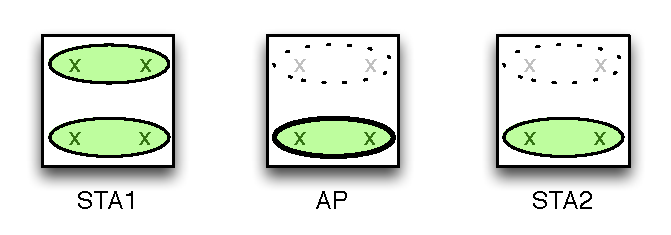
\includegraphics[width=0.5\textwidth]{images/snif2b.pdf} 	\label{fig:snif2b} }
		\subfloat[]{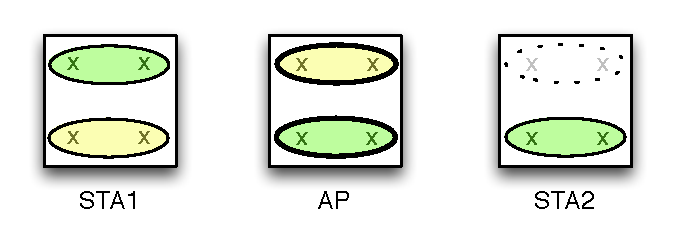
\includegraphics[width=0.5\textwidth]{images/snif2c.pdf} 	\label{fig:snif2c} }
		\caption{Third party scanning} 
	
	\end{center}
\end{figure}

\begin{exercise}{Third party scanning}
	\label{ex:secondAP}
	
So far, we only sniffed the network on nodes which took part of the network activity. Let's introduce another party, which just wants to listen to what is happening on the channel. Imagine a notebook eavesdropping on the traffic of a wireless cell. First we will add it to the same \ac{essid} and later on change it to a different \ac{essid}.  The intended setups are shown in figure \ref{fig:snif2b} and \ref{fig:snif2c}. The first situation then compares to a situation where a laptop is connected to your home network and is sniffing the traffic of other active stations in this network, while the latter situation can be seen as you being connected to your network, trying to sniff the network of a neighbour on the same channel, but using a different network name.
	
	We'll start from the previous setup.\newline
	\remark It is essential that you bring \incommand{wlan1} down on \ac{sta}1 first. 

	\begin{enumerate}
		\item Bring \incommand{wlan1} down on \ac{sta}1.\newline
		\command{\prompt{\ac{sta}1} ifconfig wlan1 down}
		\item Add \incommand{wlan0} of \ac{sta}1 to get the setup of \ref{fig:snif2b}: \newline
		\command{\prompt{\ac{sta}1} ifconfig wlan0 up}
		\command{\prompt{\ac{sta}1} iw dev wlan0 connect essid wmn-\acs{gid}-A}
		\command{\prompt{\ac{sta}1} ip addr add fc00:grID::1/64 dev wlan0}
		\item Now, reintroduce \incommand{wlan1} of \ac{sta}1 to the network.\newline
		\command{\prompt{\ac{sta}1} ifconfig wlan1 up}
		\command{\prompt{\ac{sta}1} iw dev wlan1 connect wmn-\acs{gid}-A}
		\item Configure \incommand{wlan1} with the following IP address:\newline
		\command{\prompt{\ac{sta}1} ip addr add fc00:grID:1::1/64 dev wlan1}
		\remark Remark that this IP address belongs to a different subnet! This is in preparation of the next part of the exercise.
		\item Repeat steps \ref{ex:1-1} to \ref{ex:1-3} from exercise \ref{ex:firstScan} , but in step 2, start the capture only on \incommand{wlan1} of \ac{sta}1 and save it to \file{\acs{sta}1.A.pcap}.
		\item To change the \verb!wlan1! interface to another \ac{essid}, we first need another \ac{ap} managing this \ac{essid} (figure \ref{fig:snif2c}). Configure a second \ac{ap} interface on the \ac{ap} node, this time using ``\ac{wmn}-\ac{gid}-B'' as essid\\
		\remark Copy the previous hostapd.conf file and change the ssid and interface.
		\item Make sure \verb!wlan1! of \ac{sta}1 is connected to the \ac{wmn}-\ac{gid}-B network.
		\item Repeat the same exercise again, saving the trace to \file{\acs{sta}1.B.pcap}. \newline
		\item Compare the results from both tests. How do these two setups compare to a wired setup?\newline
		\begin{esolution}
		\end{esolution}
	\end{enumerate}
	
\end{exercise}


\begin{exercise}{Pinging the \ac{ap}}

In the previous exercises, we have used the \ac{ap} only as a L2 device. The \ac{ap} can of course also be configured as a L3 device. We will now configure the \ac{ap} as a L3 device and perform the same ping test again, but this time from \ac{sta}1 to \ac{ap}.
	\begin{enumerate}
		\item Add an IP address on \incommand{wlan0} of the \ac{ap}: \newline
		\command{\prompt{\ac{ap}} ip addr add fc00:grID:1::3/64 dev wlan0}
		\item On \ac{sta}1, start a packet capture on \incommand{wlan1} and save it to \file{\acs{sta}1.pcap}. \newline
		\command{\prompt{\ac{sta}1} tcpdump -i wlan1 -w \file{\acs{sta}1.pcap}} 
		\item Start a ping session from \ac{sta}1 to \ac{ap}. Limit the ping to only two requests. \label{ex:1-3}\newline
		\command{\prompt{\ac{sta}1} ping6 -c 2 fc00:grID:1::3} 
		\item In the trace files, do you observe duplicate entries? Why or why not?\newline
		\begin{esolution}
		\end{esolution}
	\end{enumerate}

\end{exercise}


\begin{exercise}{Sniffing in monitor mode}

\begin{figure}[h]
	\begin{center}
		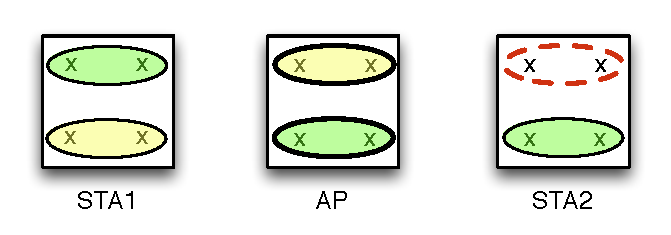
\includegraphics[width=0.5\textwidth]{images/snif4.pdf} 
		\caption{Introducing a monitoring interface.}
		\label{fig:snif4} 
	\end{center}
\end{figure}

Until now, not much difference has been observed compared to network sniffing on a wired network - apart from observing duplicate packets. In the next exercises we will broaden the setups to show the actual differences. Firstly, the monitor interface will be introduced. Configuring a \acl{wnic} in monitor mode will enable you to see all traffic that is present in a certain channel. In figure \ref{fig:snif4} the next setup is shown. We continue from the previous setup and add an extra interface.
\begin{enumerate}
	\item Configure the monitoring device:\newline
	\command{\prompt{\ac{sta}2} iw dev wlan0 set type monitor}
	\item Bring the monitor interface up: \newline
	\command{\prompt{\ac{sta}2} ifconfig wlan0 up} 
	\item Configure the channel: \newline
	\command{\prompt{\ac{sta}2} iw dev wlan0 set channel x} 
	\remark Remark that it is not necessary to configure an \ac{essid}. Why?\newline
	\begin{esolution}
	\end{esolution}
	\item Clear the \ac{nd} caches:\newline
	\command{\prompt{\ac{sta}2} ip neigh flush dev wlan1}
	\command{\prompt{\ac{sta}1} ip neigh flush dev wlan0} 
	\item Start a capture session on the monitor interface and save it to \file{\acs{sta}2.pcap}:\newline
	\command{\prompt{\ac{sta}2} tcpdump -i wlan0 -w \file{\acs{sta}2.pcap}} 
	\item Start a ping session from \ac{sta}1 to \ac{sta}2. \label{ex:3-4}\newline
	\command{\prompt{\ac{sta}1} ping6 -c 2 fc00:\acs{gid}::2} 
	\item Open the capture file in Wireshark. 
	\begin{itemize}
		\item What type of frames are visible within the trace? Give an example (packet number) of each. \newline
		\begin{esolution}
		\end{esolution}
		\item What type of link layer headers  are visible now?\newline
		\begin{esolution}
		\end{esolution}
		\item A radiotap header should also be visible before the link layer header. This header is not actually transmitted, but is used to communicate transmission statistics between the driver and kernel. As such, it reports on various transmission statistics as the signal strength and the used antenna. Select a packet (give the packetID within the trace), and list which items are present. Although the format is standardized, the actual content depends on the driver and hardware used.\newline
		\begin{esolution}
		\end{esolution}
		\item Describe the path a packet takes to be delivered from one \acl{sta} to another. Give a detailed overview of the various addresses in the headers. Identify the frames (packet ID) from the trace you use to illustrate this.\newline
		\begin{esolution}
		\end{esolution}
	\end{itemize}
\end{enumerate}
\end{exercise}


Remember the traces you made containing duplicate packets? The duplicates can now be clearly observed in the traces from a monitor interface. Each transmission from one \acl{sta} to another, both connected to the same \ac{ap} is always relayed over the \ac{ap}. The sender thus first recorded its transmission and then detected the relayed frame on the air. Frames which are sent to an \ac{ap}, are discarded by other stations. This explains why a third station did not show duplicate packets. Finally, an \acl{ap} will only report one occurrence in \incommand{tcpdump} traces, as the relaying of a frame is done transparently to the kernel in the hardware/driver.


\begin{exercise}

Finally, we will repeat exercise \ref{ex:secondAP}. We will be sending traffic on both wireless networks and monitor the channel. The setup remains unchanged (see figure \ref{fig:snif4}).

\begin{enumerate}
	\item Clear the \ac{nd} caches as before. Be sure to delete all \ac{nd} entries on all \acp{wnic}!
	\item Start a scan on the monitor interface of \ac{sta}2 and save it to \file{\acs{sta}2.pcap}: \newline
	\command{\prompt{\ac{sta}2} tcpdump -i wlan0 -w \file{\acs{sta}2.pcap}}
	\item Perform a ping from \ac{sta}1 to \ac{ap} and start a ping from \ac{sta}2 to \ac{sta}1, both on \incommand{wlan1}. This means we will inject traffic on both wireless networks.\newline
	\remark These pings can be performed consecutively. Make sure they are in the same capture session. \newline
	\command{\prompt{\ac{sta}1} ping6 -c 2 fc00:\acs{gid}:1::3}
	\command{\prompt{\ac{sta}2} ping6 -c 2 fc00:\acs{gid}::1}
	\item Which ping session(s) is/are visible in the trace?\newline
	\begin{esolution}
	\end{esolution}
\end{enumerate}




\end{exercise}





\section{Ad-Hoc Networks}

In the next section, we will set up a basic ad-hoc network. Contrary to the infrastructure network we used in the previous section, ad-hoc networks are built from identically configured hosts, without a central entity in charge. Let's start right away to build our first ad-hoc network.

\begin{exercise}{Basic ad-hoc network}

\begin{enumerate}
	\item To ensure all interfaces are in the default state, reboot all devices:\newline
	\command{\prompt{\ac{ap}} reboot}
	\command{\prompt{\ac{sta}1} reboot}
	\command{\prompt{\ac{sta}2} reboot}
	\item  The basic setup is shown in figure \ref{fig:ad-hoc1}. All nodes will have the same configuration: mode, \ac{essid} and channel.\newline
	\command{\prompt{\ac{sta}1} iw dev wlan1 set type ibss}
	\command{\prompt{\ac{sta}2} iw dev wlan1 set type ibss}
	\command{\prompt{\ac{sta}3} iw dev wlan1 set type ibss}
	\begin{figure}
		\begin{center}
			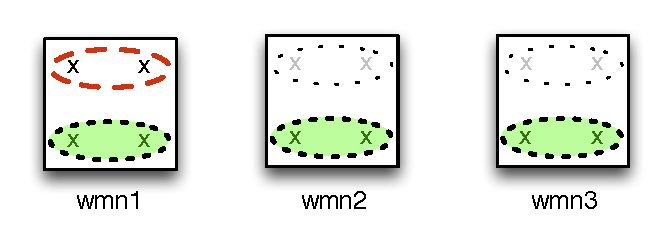
\includegraphics[width=0.5\textwidth]{images/adhoc1.pdf} 
			\caption{Basic ad-hoc network.}
			\label{fig:ad-hoc1} 
		\end{center}
	\end{figure}
	\item Assign IP addresses to all interfaces and activate them:\newline
	\command{\prompt{\ac{sta}1} ip addr add fc00:\acs{gid}::1/64 dev wlan1}
	\command{\prompt{\ac{sta}2} ip addr add fc00:\acs{gid}::2/64 dev wlan1}
	\command{\prompt{\ac{sta}3} ip addr add fc00:\acs{gid}::3/64 dev wlan1}
	\command{\prompt{\ac{sta}1} ifconfig wlan1 up}
	\command{\prompt{\ac{sta}2} ifconfig wlan1 up}
	\command{\prompt{\ac{sta}3} iwconfig wlan1 up}
	\item Configure all interfaces with a \ac{essid} and a channel:\newline
	\command{\prompt{\ac{sta}1} iw dev wlan1 ibss join \ac{wmn}-\acs{gid}-A <frequency>}
	\command{\prompt{\ac{sta}2} iw dev wlan1 ibss join \ac{wmn}-\acs{gid}-A <frequency>}
	\command{\prompt{\ac{sta}3} iw dev wlan1 ibss join \ac{wmn}-\acs{gid}-A <frequency>}
	\remark The frequency you should use here can be found in the introduction section.\newline
	\item To monitor the traffic in the channel, set up a monitor interface on \ac{sta}1:\newline
	\command{\prompt{\ac{sta}1} iw dev wlan0 set type monitor}
	\command{\prompt{\ac{sta}1} ifconfig wlan0 up}
	\command{\prompt{\ac{sta}1} iw dev wlan0 set freq <frequency>}
	\item Scan using the monitor interface and save it to \file{\acs{sta}1.pcap}.\newline
	\command{\prompt{\ac{sta}1} tcpdump -i wlan0 -w \file{\acs{sta}1.pcap}}
	\item Verify that the nodes now all can reach each other:\newline
	\command{\prompt{\ac{sta}1} ping6 -c 2 fc00:\acs{gid}::2}
	\command{\prompt{\ac{sta}2} ping6 -c 2 fc00:\acs{gid}::3}
	\command{\prompt{\ac{sta}3} ping6 -c 2 fc00:\acs{gid}::1}	
	\item Describe how data is exchanged between the various hops. How does this compare to infrastructure mode? Motivate your findings by selecting frames (give the packet ID) from the trace file and describe their \ac{mac} header and addressing scheme.\newline
	\begin{esolution}
	\end{esolution}
	
	\item Repeat the ping tests from exercise \ref{ex:pingtest} (from \ac{sta}1 to \ac{sta}2 and write down the requested values. Do you observe a significant change in timings?\newline
	\begin{esolution}
	\end{esolution}
\end{enumerate}
	
\end{exercise}
%%!TEX root = labo.tex
\setcounter{chapter}{1}
\chapter{Frequencies and Channels}

In the \wifi standards, various channels are defined. Two main frequency bands are used, namely 2.4 GHz and 5GHz. \wifi{a} networks use the 5 GHz band, while \wifi{b/g} networks operate in the 2.4 GHz band. In both bands, various ``channels'' have been defined. However, channel separation is not as clean cut as one might expect. In the following setups, you will illustrate this using some simple tests.

\section{Available channels}
\begin{exercise}{Frequencies}

Within the \wifi specification, various channels are defined. Depending on the local authorities (\ac{bipt} in Belgium\cite{bipt}), the list of allowed channels can vary. Using \incommand{iw} you can get the list of available channels.\newline
\remark The wireless drivers we use make a difference between the logical interface (\incommand{wlan0} as we have used it so far) and the actual physical radio interface. All things related to physical characteristics are actually handled by the physical interface, which is called \incommand{phy0} or \incommand{phy1}, respectively.\newline
\begin{enumerate}
	\item  To get a correct overview of which frequencies/channels are available in Belgium, use the command \incommand {iw phy1 info}.
	\item List all frequencies/channels that the \incommand{phy1} interface supports.\newline
	\begin{esolution}
	\end{esolution}
\end{enumerate}

You should observe several frequencies that are marked \emph{disabled}. This indicates that the card supports these frequencies, but cannot use them because of Belgian regulations. Also, several frequencies should be marked with \emph{radar detection}. These can be used, but special mechanisms must be put in place in order to avoid interference with radar installatiuons (e.g. airport radar).

\end{exercise}

\begin{exercise}{Available UA hotspots}
\begin{figure}[h]
	\begin{center}
		
		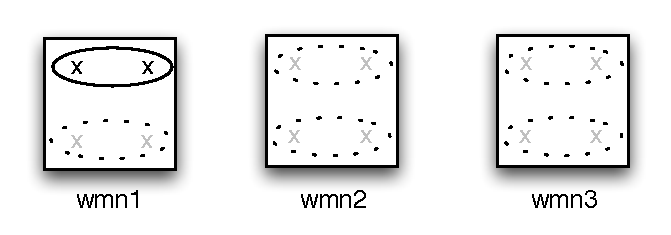
\includegraphics[width=0.5\textwidth]{images/channels1.pdf}
		\caption{Channel separation setup 1} 
		\label{fig:channels1} 
	\end{center}
\end{figure}

\begin{enumerate}
		\item Start by building the setup as illustrated in figure \ref{fig:channels1}. \newline
		\remark Remark that it is not necessary to configure the SSID or channel, but bring up the interface to activate it.
		\item Find out which \acp{ap} are active using \incommand{iw wlan0 scan}. This command provides an interface to list various settings from the \ac{wnic}. The manpage or command line help should be self-explanatory.
		\item Fill in the following table:\newline
		\begin{esolution}
		\end{esolution}
\ifthenelse{\not \boolean{Solutions}}{
		\renewcommand\arraystretch{2.5}
		\setlength\LTleft{0pt}
		\setlength\LTright{0pt}

		\begin{longtable}{@{\extracolsep{\fill}}ccc}
		%{\textwidth}{@{\extracolsep{\fill}}
		\hline
		SSID & Frequency (MHz) & BSS \\
		\hline
		& & \\
		\hline
		& & \\
		\hline
		& & \\
		\hline
		& & \\
		\hline
		\end{longtable}}{}
%		\item \report Write down the exact command used to obtain your results:
%		\begin{esolution}{2}
%		\end{esolution}
	\end{enumerate}
\end{exercise}

\section{Channel Separation}

\begin{exercise}{Channel overhearing} \label{ex:overhearing}
	
	\begin{figure}[h]
		\begin{center}
			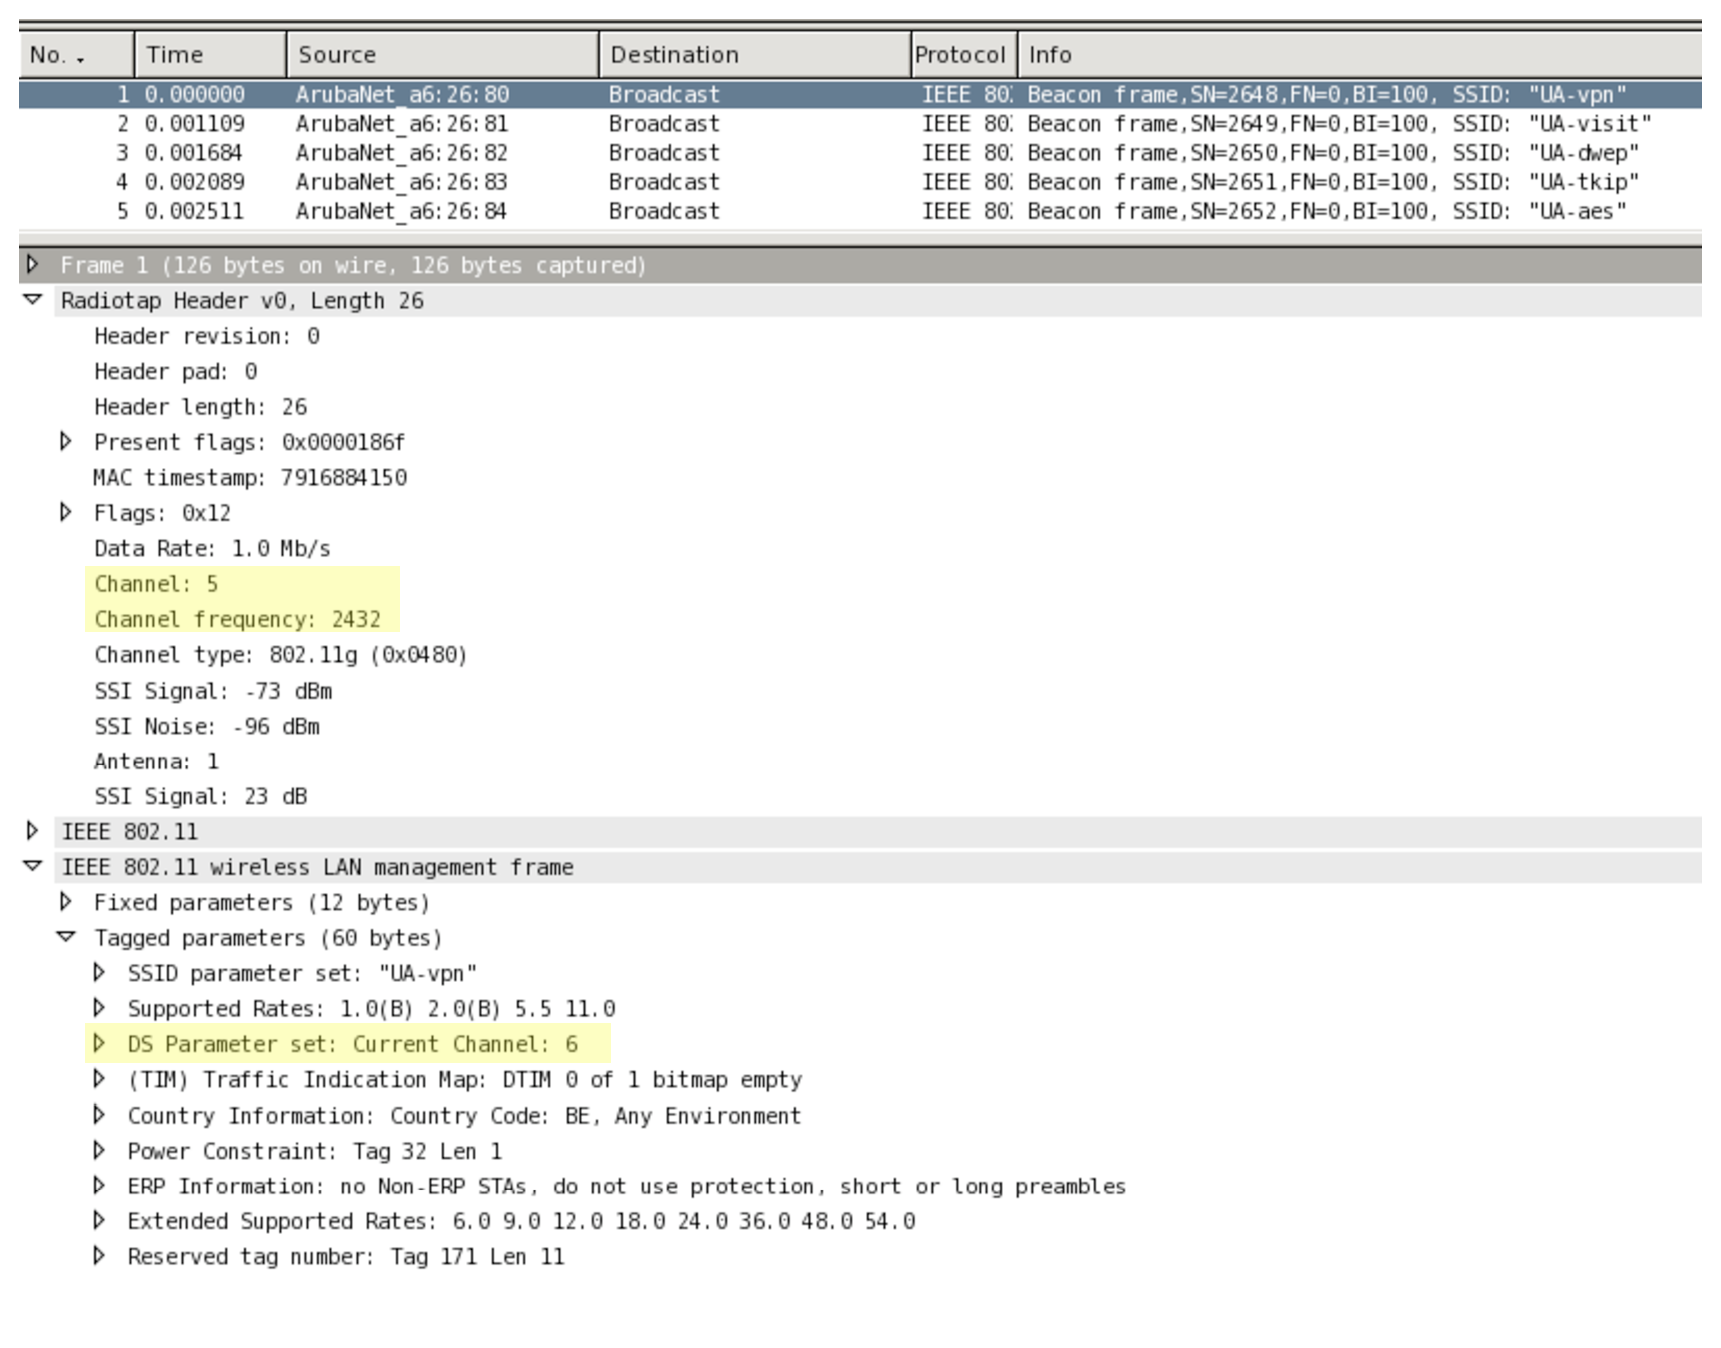
\includegraphics[width=\textwidth]{images/beacon.pdf}
			\caption{Channels in a captured beacon frame.} 
			\label{fig:beacons} 
		\end{center}
	\end{figure}
	
	
In the previous exercise, you made an overview of a lot of \aclp{ap}. The next exercise will illustrate the channel overhearing. The information about which channel an \ac{ap} is working on, is provided in the beacon frames the \ac{ap} periodically transmits. In figure \ref{fig:beacons}, a Wireshark\cite{wireshark} screen shot shows a beacon frame. The Radiotap header indicates the frame was received on channel 5, while the beacon's content shows the \ac{ap} sending this beacon only operates at channel 6. Channels are thus not cleanly separated.  In the next exercise you'll create an overview of the channel overhearing.

\begin{figure}[h!]
		\begin{center}
			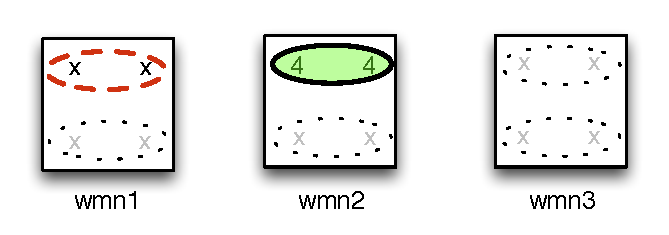
\includegraphics[width=0.5\textwidth]{images/channels2.pdf}
			\caption{Setup for exercise \ref{ex:overhearing}.} 
			\label{fig:channels2} 
		\end{center}
\end{figure}
	
	\begin{enumerate}
		\item Start from the setup as shown in figure \ref{fig:channels2}. \newline
		\remark Note that the \ac{ap} should be configured in channel 4 from the b/g range. To be able to do this, you should change the line \verb!hw_mode=a! to \verb!hw_mode=b! in the hostapd.conf file.
		\item On \ac{sta}1, on every channel, make a capture \file{chanID.pcap}.\newline
		\item Use the following wireshark display filter to only show beacons:\newline
		\command{wlan.fc.type\_subtype == 8}
		\item Fill out the following table using the obtained information.\newline
		\begin{esolution}
		\end{esolution}
		

\ifthenelse{\not \boolean{Solutions}}{
\begin{longtable}{@{\extracolsep{\fill}}c|l}	
	Selected channel & Observed channels in received beacons \\
	\hline
	1&\\\hline
	2&\\\hline
	3&\\\hline
	4&\\\hline
	5&\\\hline
	6&\\\hline
	7&\\\hline
	8&\\\hline
	9&\\\hline
	10&\\\hline
	11&\\\hline
\end{longtable}	}{}
		\end{enumerate}
\end{exercise}

\begin{figure}[h!]
	\begin{center}
		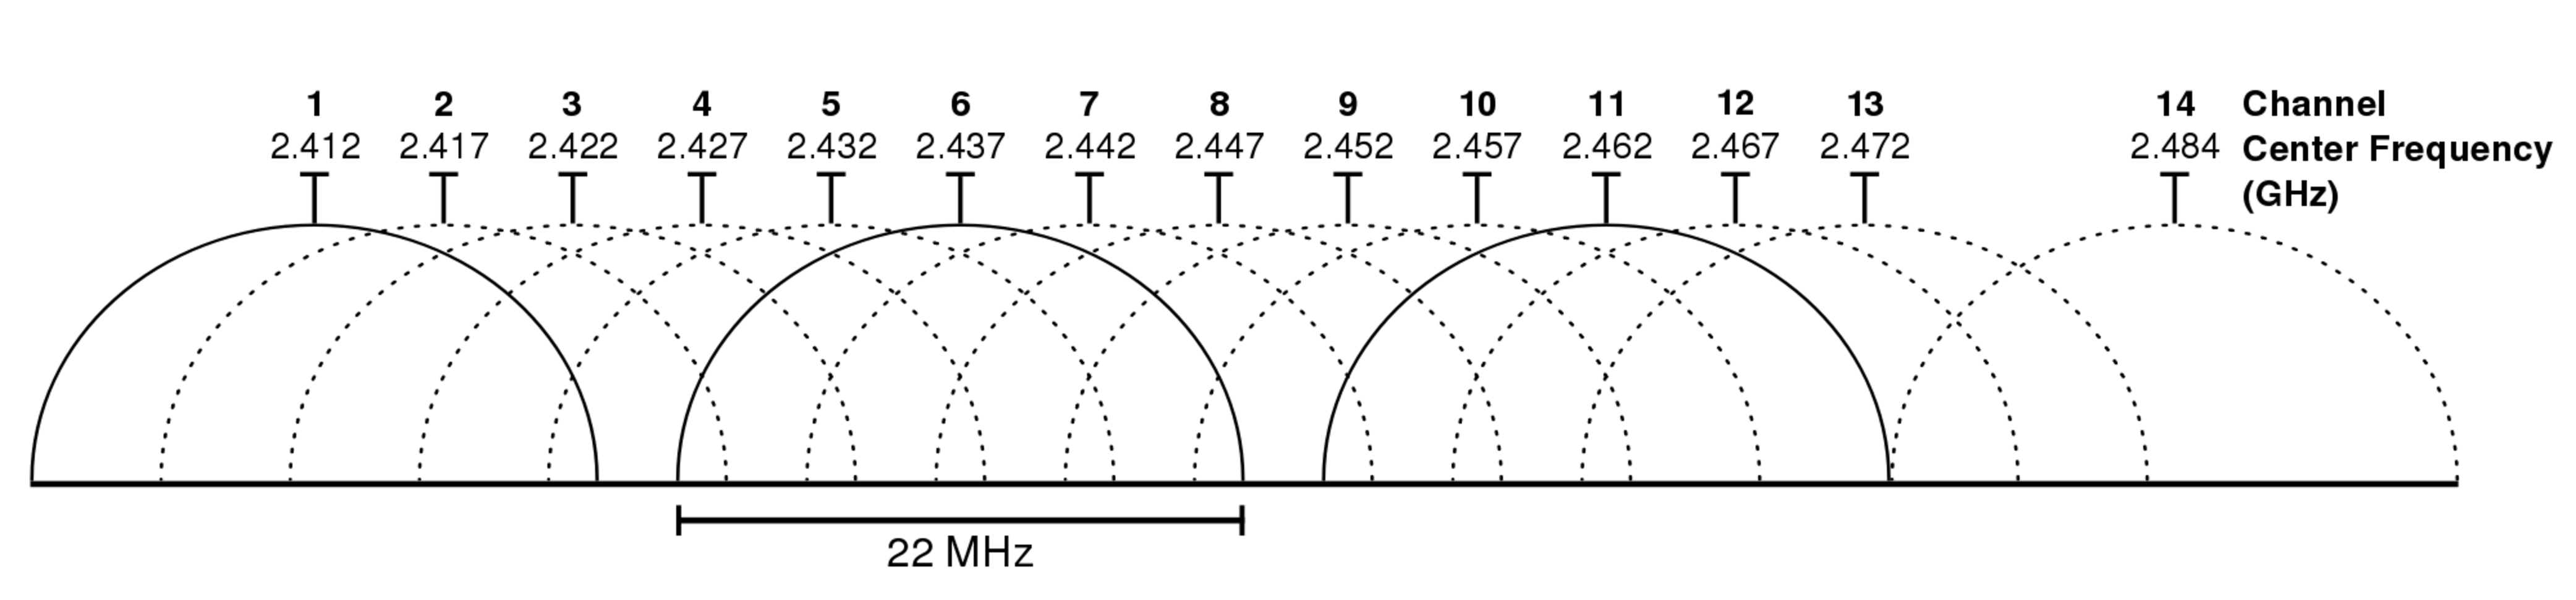
\includegraphics[width=\textwidth]{images/bgchannels.pdf}
		\caption{2.4 GHz channels} 
		\label{fig:channel_separation} 
	\end{center}
\end{figure}

From this exercise, it should be clear that the channels within the \wifi{b/g} range are not strictly separated.  Figure \ref{fig:channel_separation}\footnote{By Michael Gauthier, Wireless Networking in the Developing World [CC-BY-SA-3.0 (http://creativecommons.org/licenses/by-sa/3.0)], via Wikimedia Commons} gives you an idea why: the consecutive channels overlap to a certain extent. Therefore, a careful channel planning is crucial in building and deploying wireless networks on these frequencies. In the next exercise, we will take a look at the channel separation in the \wifi{a} band.

\begin{exercise}{Channel separation in \wifi{a}}\label{ex:separation}
	
	\begin{enumerate}
		\item Now, change the \ac{ap} so that it is on channel \verb!x!.
		\item Using \incommand{tcpdump} as in the previous exercise, find out in which channels \wifi{a} the beacons of this \ac{ap} can be seen. Save your traces in \file{chanID.pcap}.\newline
		\begin{esolution}
		\end{esolution}
	\end{enumerate}
	
\end{exercise}

\section{Using the Wireless Channel}

\begin{figure}[h]
		\begin{center}
			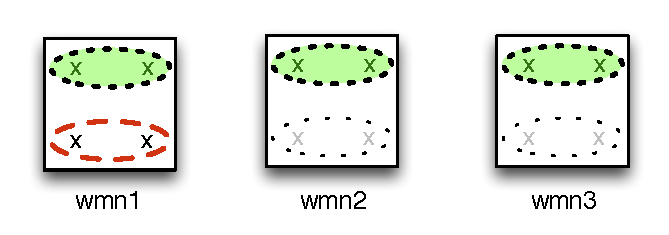
\includegraphics[width=0.5\textwidth]{images/adhoc2.pdf} 
			\caption{Basic ad-hoc network.}
			\label{fig:ad-hoc2} 
		\end{center}
	\end{figure}
	
\begin{exercise}{Beacons}

In the next few exercises, we will again use an ad-hoc network setup. It is best to reboot the devices before proceeding.
\begin{enumerate}
	\item Create the network setup as shown in figure \ref{fig:ad-hoc2}. Perform the following commands on all three stations. Substitute \incommand{nodeNumber} with a different number (e.g. 1, 2 and 3) on each node.\newline
		\command{\prompt{wmn} iw dev wlan0 set type ibss}
		\command{\prompt{wmn} ip addr add fc00:\acs{gid}::nodeNumber/64 dev wlan0}
		\command{\prompt{wmn} ifconfig wlan0 up}
		\command{\prompt{wmn} iw dev wlan0 ibss join \acs{wmn}-\acs{gid}-A <frequency>}
	\item Put interface wlan1 of \ac{sta}1 in monitor mode on the same frequency.\newline
		\command{\prompt{\ac{sta}1} iw dev wlan1 set type monitor}
		\command{\prompt{\ac{sta}1} ifconfig wlan1 up}
		\command{\prompt{\ac{sta}1} iw dev wlan1 set freq <frequency>}
	\item Check if all stations can reach each other.
	\item Perform a \incommand{tcpdump} on the monitor interface. Save it to \file{\acs{sta}1.pcap}. Let it run for a few seconds and then stop the trace.
	\item In your trace file, you should observe beacon frames. Carefully inspect one of the beacon frames in this trace and compare it to a beacon frame captured in the previous exercise (exercise \ref{ex:separation}). Give the packet IDs of the beacon frames you are comparing and identify the differences in the management frame part.\newline
	\begin{esolution}
	\end{esolution}
	\item Start a new trace on the monitor interface and save it to \file{STA1.pcap}.
	\item While the trace is running, perform two ping tests. You may perform the simultaneously, but it will be easier to answer the next question if you perform them consecutively.\newline
	\command{\prompt{\ac{sta}2} ping6 -c 5 fc00:\acs{gid}::3}
	\command{\prompt{\ac{sta}3} ping6 -s 1400 -c 5 fc00:\acs{gid}::1}
	\item Open your trace file and filter out the beacon frames with the following display filter: \verb#!(wlan.fc.type_subtype == 0x08)#. Apart from the data frames, which kind of frames do you observe?\newline
	\begin{esolution}
	\end{esolution}
	\item Explain the purpose of those frames.\newline
	\begin{esolution}
	\end{esolution}
\end{enumerate}
\end{exercise}

\begin{exercise}{\ac{rts}/\ac{cts}}

For this exercise, you will study the \ac{rts}/\ac{cts} mechanism. This mechanism will clear the channel for each transmission, minimizing the chance of collisions in the channel. A threshold value is used to determine if \ac{rts}/\ac{cts} should be used. Larger packets will receive \ac{rts}/\ac{cts} protections while smaller packet will not. Using \ac{rts}/\ac{cts} for small packets adds a lot of overhead and hence degrades performance.

\begin{enumerate}
	\item Start from the setup as for the previous exercise.
	\item The \ac{rts}/\ac{cts} threshold will be set with \incommand{iwconfig wlan0 rts 1000}. Perform this command on all nodes.
	\item Performing the same \incommand{ping6} commands as in the previous exercise. Start a capture session on the monitor interface and save it to \file{STA1.pcap}.
	\item You should observe \ac{rts}/\ac{cts} packets. Which packets are protected by this mechanism? Give an example (packet ID).\newline
	\begin{esolution}
	\end{esolution}
	\item Compare an \ac{rts} and \ac{cts} frame. How do they differ? Illustrate using frames from your last trace file.
	\begin{esolution}
	\end{esolution}
\end{enumerate}

As you can see in the \ac{rts}/\ac{cts} frames, they do not contain any information about the network on which they are transmitted. The \ac{rts}/\ac{cts} is meant to avoid collisions on the wireless medium, so any node that receives a \ac{cts} frame is required to remain silent for the duration included in the \ac{cts} frame. The only exception, for obvious reasons, is the node to which the \ac{cts} frame is sent. Capturing \ac{rts}/\ac{cts} frames (or acknowledgement frames) on a certain channel is always a good indication that some activity is going on in that channel, even if it is impossible to overhear the actual data transmission.
\end{exercise}

\section{\wifi{n}}


Until now, we have only used the \acp{wnic} in \wifi{a} or b/g mode. ``b'' is the oldest mode. ``g'' improves upon ``b'' by offering significantly higher maximal throughput (54 Mbps versus 11 Mbps) .``a'' operates at different frequencies and offers the same throughput as ``g''.

Another mode of operation is called ``n''. \wifi{n} is an amendment to the \wifi standard in order to improve throughput over both ``a'' and ``g''. It operates at both frequency bands and is defined for bit rates up to 600 Mbps, but very few setups will be able to obtain these speeds.

\wifi{n} can use different optimizations, such as the \ac{mimo} principle, 40 MHz wide channels (versus 20 MHz in \wifi{a/b/g}), and frame aggregation to improve throughput. The following exercise will demonstrate that \wifi{n} channels can indeed be twice as wide as those in \wifi{a}, and thus interfere with adjacent \wifi{a} channels.

\begin{exercise}{\wifi{n}}

\begin{figure}[h]
		\begin{center}
			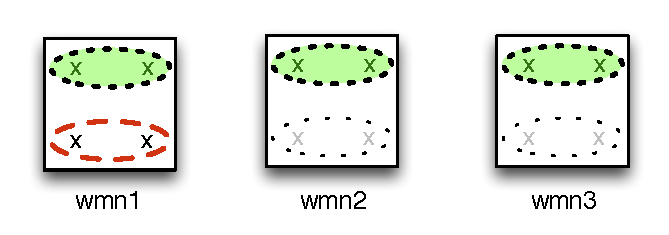
\includegraphics[width=0.5\textwidth]{images/adhoc2.pdf} 
			\caption{\wifi{n} ad-hoc network.}
			\label{fig:ad-hoc-n} 
		\end{center}
	\end{figure}

\stress{As this exercise will use both channels allocated to the mobile and wireless lab, two groups cannot perform this exercise at the same time! Check if no other group is currently working on this course!} 

\begin{enumerate}
	\item Reboot all devices. In order to enable \wifi{n} mode without any problems, we will start from a blank setup.
	\item After they have been rebooted, perform the following on all devices in order to create an ad-hoc network with \wifi{n} support in the 5 GHz band:\newline
		\command{\prompt{\ac{sta}} iw dev wlan0 set type ibss}
		\command{\prompt{\ac{sta}} ip addr add fc00:\acs{gid}::nodeNumber/64 dev wlan0}
		\command{\prompt{\ac{sta}} ifconfig wlan0 up}
		\command{\prompt{\ac{sta}} iw dev wlan0 ibss join wmn-\acs{gid}-A 5180 HT20}
	\item Check that all nodes can reach each other.
	\item Set up a monitor interface on channel 36 (5180 MHz) on \ac{sta}1.
	\item Start a trace on the monitor interface and save it to \file{\acs{sta}1.pcap}.
	\item Start a ping from \ac{sta}2 to \ac{sta}3 and from \ac{sta}3 to \ac {sta}1. Like before, use different ping sizes:\newline
		\command{\prompt{\ac{sta}2} ping6 -c 5 fc00:\acs{gid}::3}
		\command{\prompt{\ac{sta}3} ping6 -s 1400 -c 5 fc00:\acs{gid}::1}
	\item Filter out the beacon frames from your trace. Do you observe packets from both ping sessions? Did you see all packets from these sessions? Why or why not?\newline
	\begin{esolution}
	\end{esolution}
	\item Set the monitor interface to channel 40 (5200 MHz).
	\item Perform the same ping test again, but now save your trace to \file{\acs{sta}1.pcap}.
	\item Did you capture any packets?\newline
	\begin{esolution}
	\end{esolution}
\end{enumerate}

	
\end{exercise}

\begin{exercise}{40 MHz channels}

In the previous exercise, we enabled \wifi{n}, but we did not enable 40 MHz wide channels yet. We will do that now.
\begin{enumerate}
	\item Deconfigure all \incommand{wlan0} interfaces.\newline
	\command{\prompt{\ac{sta}} iw dev wlan0 ibss leave}
	\item Now, create an ad-hoc network that uses 40 MHz wide channels:\newline
	\command{\prompt{\ac{sta}} iw dev wlan0 ibss join wmn-0-A 5180 HT40+}
	\item As in the previous exercise, set the monitor interface of \ac{sta}1 on channel 36 and perform a capture while sending both pings. Save it to \file{\acs{sta}1.36.pcap}.
	\item Do the same again, but this time monitor channel 40.\newline Save your trace in \file{\acs{sta}1.40.pcap}.
	\item Do you observe any different behaviour in the trace file on channel 36, compared to the previous exercise?\newline
	\begin{esolution}
	\end{esolution}
	\item In the trace file on channel 40, which packets have you captured? Why?\newline
	\begin{esolution}
	\end{esolution}
\end{enumerate}
\end{exercise}

%%!TEX root = labo.tex
\setcounter{chapter}{2}
\chapter{Performance Measurements}

In this lab, the performance and throughput in wireless networks will be investigated. Using tools like \incommand{iperf}, we will record the maximum throughput which can be achieved in wireless networks and have a look at the parameters influencing this throughput. 

\section{Bit Rates}

\begin{exercise}{Basic throughput in \wifi{a}}\label{ex:basicTput}
\label{ex:tput1}
	
	This first exercise will give you an insight into the difference in usable throughput and the available bit rate. To determine the throughput, we will be using a tool called \incommand{iperf}. This is a client-server based tool which sends \ac{tcp} or \ac{udp} traffic and reports the measured throughput. Consult the man pages for the details about this tool. A second tool to be used is \incommand{gnuplot}, in order to plot your results in a graph. More info about \incommand{gnuplot} can be found in \cite{gnuplotHome} and a nice tutorial in \cite{gnuplotTut}. A basic gnuplot script to generate your first plots is provided on the course website. The \incommand{iperf} tool is preinstalled on the wireless nodes, while \incommand{gnuplot} is available on the lab PCs.

	\begin{figure}[h!]
		\begin{center}
			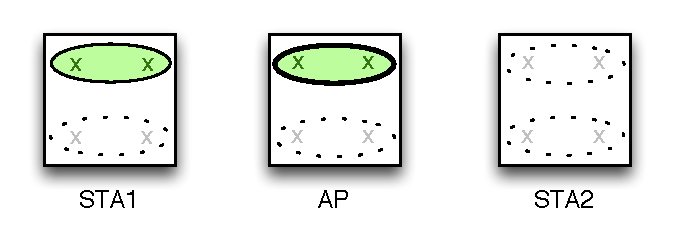
\includegraphics[width=0.5\textwidth]{images/perf1.pdf}
			\caption{Basic throughput setup.} 
			\label{fig:perf1} 
		\end{center}
	\end{figure}
	
	\begin{enumerate}
		\item Start by configuring the setup as shown in figure \ref{fig:perf1}. Use \incommand{fc00:\acs{gid}::3/64} for the \ac{ap} and \incommand{fc00:\acs{gid}::1/64} for \ac{sta}1.
		\item \label{item:rates}\wifi supports various bit rates. Using \incommand{iw list} you can query the supported rates:\newline
		Which rates are supported in \wifi{a}?\newline
		\begin{esolution}
		\end{esolution}
		Which rates are supported in \wifi{b/g}?\newline
		\begin{esolution}
		\end{esolution}
		\item \incommand{iperf} can be used to measure the maximum throughput between two stations. Therefore, a server is started on one end and a client connects on the other end to this server. A connection is set up and as \ac{tcp} tries to maximize the throughput on a connection, an estimate of the maximum throughput on a link can be calculated. When using \incommand{iperf} with the basic parameters, it will perform a 10 seconds test and report the achieved throughput at the client side.
		\item Start a basic \incommand{iperf} session between the \ac{sta} and \ac{ap}, with the \incommand{iperf} server on the \ac{ap}: \newline
		\command{\prompt{AP} iperf -V -s}
		\command{\prompt{STA1} iperf -V -c fc00:\acs{gid}::3 }
		Copy the output of the \incommand{iperf} client:\newline
		\begin{esolution}
		\end{esolution}
	
		\item Now, using \incommand{iperf}, collect the throughput for each available rate and write the results in a file \file{tcp.txt}. On each line, first put the rate followed by a space and then the result in Mbit/s obtained from \incommand{iperf}, e.g. \texttt{54 30} denotes that a 30Mbit/s was measured when using a rate of 54 Mbps. You can change the rate used at the \ac{sta} using \incommand{iw}, e.g. to 54Mbps, as follows:\newline
		\command{\prompt{STA1} iw dev wlan0 set bitrates legacy-5 54}
		You can check the actual used bit rate from the output of \incommand{iwconfig}:\newline
		\command{\prompt{STA1} iwconfig wlan0}
		\remark As we will be repeating the collection of these results in the following exercises, it will be easier to use some bash scripting to speed up this process. 
		A helper script can be found in the file \texttt{iperf-tcp.sh}. Change this script so it loops over the correct bitrates, and use it with the command \incommand{./iperf-tcp.sh fc00:grID::3}.\newline
		This script generates output that can be directly copied to \file{tcp.txt}
		
		
		\item \incommand{iperf} will by default use \ac{tcp} to check the connection, but it is also possible to use a unidirectional \ac{udp} stream. Therefore, one can try to feed more data to the network than the network can support and as such measure how much can be actually delivered. Thus, repeat the previous scenario and collect the maximum achievable throughput using \incommand{iperf} in \ac{udp} mode for each available bit rate. Save these results in the same format as in the previous item in a file \file{udp.txt}.\newline Again, a script called \texttt{udp.sh} is provided that automates this process. The script will try to send a UDP stream that fills the wireless link.\newline
		\command{\prompt{AP} iperf -V -s -u -l 1452}
		\command{\prompt{STA1} ./iperf-udp fc00:grID::3}
		\remark \texttt{-l} is the letter l, not the number one!

		\item Now plot these results using \incommand{gnuplot}. On the course website, a \incommand{gnuplot} script, \texttt{tput1.gnuplot}, is provided to plot the throughput and the relative link usage over the various available rates. The used commands are straightforward and the script is inline commented so should be self-explanatory. Make sure you understand the various commands in the file. The script produces two PDF files which can be viewed with any regular PDF viewer. Place the \texttt{.txt} files you created in the previous steps in the same directory as the \incommand{gnuplot} script. Save the generated files in your lab report as \texttt{L3-1-4-tput.pdf} and \texttt{L3-1-4-usage.pdf}. Add the plots here and shortly discuss what can be observed. Also shortly discuss the difference between \ac{udp} and \ac{tcp}. To generate the PDF files, use:\newline
		\command{gnuplot tput.gnuplot}
		\begin{esolution}
		\end{esolution}
		\end{enumerate}
\end{exercise}

\begin{exercise}{Client to client throughput}
\label{ex:tput2}
	\begin{figure}[h!]
		\begin{center}

			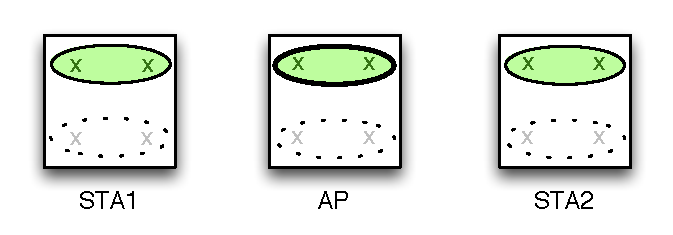
\includegraphics[width=0.5\textwidth]{images/perf2.pdf}
			\caption{Client to client throughput setup.} 
			\label{fig:perf2} 
		\end{center}
	\end{figure}
	
	In the previous exercise, the throughput was measured between a \ac{sta} and the \ac{ap} it was connected to. In this exercise, we are interested in the throughput between two \acp{sta} associated with the same \ac{ap}.
	\begin{enumerate}
		\item Create the test setup as shown in figure \ref{fig:perf2}. Configure \acs{sta}2 with IP address \texttt{fc00:grID::2/64}.
		\item Collect the \ac{tcp} and \ac{udp} throughput measures as in the previous exercise and save them to \file{tcp.txt}\\ and \file{udp.txt}.
		\item Adapt the provided \incommand{gnuplot} script and create graphs for the new measurements. Include them in your report.
		\item Comment on the obtained results and compare the results from this exercise with those from the previous exercise. Explain the difference.\newline
		\begin{esolution}
		\end{esolution} 
	\end{enumerate}
	
\end{exercise}

\section{Network Settings}
\begin{exercise}{\acs{rts}/\acs{cts}}

In lab 2, we enabled the \ac{rts}/\ac{cts} mechanism to show that in \wifi, stations can reserve the medium in order to avoid collisions. In this exercise, we will study the effect of \ac{rts}/\ac{cts} on throughput.

\begin{enumerate}
	\item Enable \ac{rts}/\ac{cts} on all devices.\newline
	\command{\prompt{} iw phy phy0 set rts 1000}
	\item Repeat the iperf tests from \ac{sta}1 to \ac{ap}. Save your logs to \file{tcp.txt}\\ and \file{udp.txt}. Again modify the gnuplot script to create new graphs and include them in your report. To make the comparison more easy, modify the gnuplot script so that you plot both the results from exercise \ref{ex:tput1} and this exercise on the same graph. What do you observe? Why?\newline
	\begin{esolution}
	\end{esolution}

\end{enumerate}

\end{exercise}

\begin{exercise}{Frame length}

	The standard \ac{mtu} for ethernet frames is 1500 bytes. \wifi however allows an \ac{mtu} up to 2274 bytes. In this exercise, you will measure the effect of frame size on throughput.
	
	\begin{enumerate}
		\item Continue from the previous setup, but make sure \ac{rts}/\ac{cts} is turned off on all nodes:\newline
		\command{iw phy phy0 set rts off}
		\item On \ac{sta}1, reset rate control to its default (automatic) value:\newline
		\command{\prompt{\ac{sta}1} iw dev wlan0 set bitrates}
		\item Perform the following tests with 4 different maximum frame sizes: 1500, 1758, 2016 and 2274. The frame size can be controlled by changing the \ac{mtu}. \emph{If you do this, do this on all nodes!}\newline
		\command{ifconfig wlan0 mtu 1758}
		\item For each of the \acp{mtu} mentioned, start with a \ac{tcp} \incommand{iperf} test between \ac{sta} and \ac{ap} as in the previous exercises and make plots for each frame size. Generate a results file called \file{tcp.txt}\\ containing \ac{mtu} and bit rate achieved. The file should have the same format as the ones produced this far, except that the first column now contains your \ac{mtu} setting rather than the link speed.\newline
		\command{\prompt{\ac{sta}1} iperf -V -c fc00:grID::3}
		\item Repeat the tests, now using \ac{udp}. For \incommand{iperf}, use the \incommand {-l}  parameter, followed by the current MTU setting minus 48 (e.g. 1452 if the \ac{mtu} is set to 1500) to generate packets that are large enough to fill the MTU. \stress{This must be done on both client and server!} Save your results to \file{udp.txt}\\.\newline
		\command{\prompt{\ac{sta}1} iperf -V -u -l 1452 -c fc00:grID::3 -b 54M}
    		\item Modify the \incommand{gnuplot} script to generate the same graph as before. Plotting only the throughput versus \ac{mtu} suffices. A relative link usage graph is not required. What do you observe? Why? Be as precise as possible.\newline
		\begin{esolution}
		\end{esolution}	 
	\end{enumerate}
		
\end{exercise}


\section{Packet Size}
\begin{exercise}{IP Fragmenting}

	Changing frame lengths has an effect on the throughput, as you have shown in the previous exercise. However, in that case, traffic was flowing between segments with the  same fragment size. When we consider the default setup of an \ac{ap} which is connected to the Internet, the \ac{wan} link is most likely limited to 1500 bytes per frame and thus IP fragmenting comes into play. In IPv6, fragmenting in intermediate hops is not allowed. The end hosts may, however, fragment the IP packets end-to-end to make sure they fit on the link with the smallest \ac{mtu}. Depending on the original payload length, fragments of various lengths will be created. In this exercise we will have a look at the impact of fragmenting on the overall throughput.
	
	To do so, we will run the \incommand{iperf} server on the third node, which is only connected by wire to the \ac{ap}. Using additional routes, we will create a setup where \ac{sta}1 and \ac{sta}2 communicate via the \ac{ap}. Traffic between \ac{sta}1 and the \ac{ap} will be transmitted on the wireless link, while traffic between the \ac{ap} and \ac{sta}2 will be transmitted on the wired link.
	
	\begin{figure}[h!]
		\begin{center}
			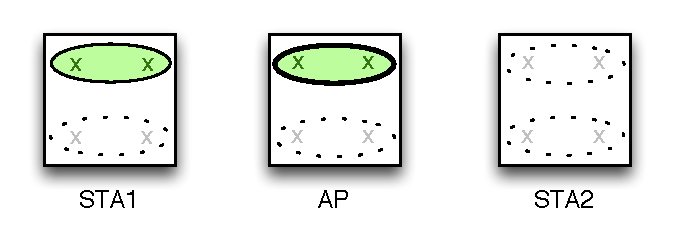
\includegraphics[width=0.5\textwidth]{images/perf1.pdf}
			\caption{Fragmenting setup.} 
			\label{fig:fragmenting} 
		\end{center}
	\end{figure}



	\begin{enumerate}
		\item Start by configuring your setup as shown in figure \ref{fig:fragmenting}. \ac{sta}2 will only be used as \incommand{iperf} server and does not need an active \ac{wnic}.
		\item Set \texttt{fc00:\acs{gid}::3/64} as IP for the \ac{ap} and \texttt{fc00:\acs{gid}::1/64} for \ac{sta}1.
		\item Traffic from \ac{sta}1 to \ac{sta}2 will by default use the wired network. To force a wireless hop, we will add some new routes:\newline
		\command{\prompt{\ac{sta}2} ip route add fc00:\acs{gid}::/64 via <wired IP address of \acs{ap}>}
		\command{\prompt{\ac{sta}1} ip route add <wired IP address of \acs{sta}2>/128 via fc00:\acs{gid}::3}
		\item IPv6 forwarding is by default not enabled on the lab nodes. We must enable it on the \ac{ap} for the setup to work. However, due to a bug, the \ac{ap} will clear its default route when we do this, making it instantly inaccessible over IPv6. Perform the following as a workaround:\newline
		\command{\prompt{\ac{ap}} ip -6 route show | grep default}
		You should get output like this:\newline
		\texttt{default via fe80::225:90ff:fe61:efac dev eth0  proto kernel  metric 1024  expires 1670sec}
		\item Enable IPv6 routing functionality on the \ac{ap}:\newline
		\command{\prompt{\ac{ap}} sysctl -w net.ipv6.conf.all.forwarding=1 \&\& ip route add default via fe80::225:90ff:fe61:efac dev eth0}\newline
		The IP address in that command should be the same as that in the output of the previous step.
		\item Perform a \incommand{traceroute6} from \ac{sta}1 to \ac{sta}2 to check if the routes are set up correctly. Include your traceroute6 output below:\newline
		\command{\prompt{\ac{sta}1} traceroute6 <wired IP address of \acs{sta}2>}\newline
		\begin{esolution}
		\end{esolution}
		\item Now, for each \ac{mtu} (1500, 1758, 2016 and 2274), perform the following:\newline
		\begin{itemize}
			\item Set the \ac{mtu} on the wireless link.
			\item Perform a TCP \incommand{iperf} from \ac{sta}1 to \ac{sta}2.
			\item Perform a UDP \incommand{iperf} from \ac{sta}1 to \ac{sta}2. In each trace, set your frame size to the \ac{mtu} of the wireless link minus 48. Send at a bit rate of 54 Mbps.
		\end{itemize}
		\item The results of your tests should once again be saved to text files like in the previous exercise. Save them to \file{tcp.txt}\\ and \file{udp.txt}\\. Create a throughput graph as in the previous exercise.
		\item You should also make \texttt{.pcap} trace files from these experiments. However, as the link gets fully saturated, the trace file would become very large. Therefore, we will repeat the experiments sending far less traffic. This of course means that you will not see a difference in \incommand{iperf} results. The traces will help you, however, to understand what has happened in the previous exercise.
		\item In order to limit the amount of traffic, we will do the following on \ac{sta}1:
		\begin{itemize}
		\item Set the rate of \texttt{wlan0} to 6 Mbps.
		\item for both TCP and UDP \incommand{iperf}, add the \texttt{-t 2} parameter. This limits the \incommand{iperf} trace to two seconds.
		\item for UDP \incommand{iperf}, omit the \texttt{-b 54M} parameter. This way, \incommand{iperf} will only transmit at 1 Mbps.
		\end{itemize}
		\item Now, do the same \incommand{iperf} tests again, using the above parameters for \incommand{iperf}. For each run, make a \incommand{tcpdump} trace on interface \texttt{wlan0} of the \ac{ap}. Save the traces to \file{tcp.<MTU size>.pcap}\\ and \file{udp.<MTU size>.pcap}\\, respectively.
		\item What do you observe? Distinguish between the behaviour for TCP and UDP. Explain your findings by including your graphs and refering to the trace files you made. Be as precise as possible.\newline
		\begin{esolution}
		
		\end{esolution}
 
	\end{enumerate}	
\end{exercise}
%%!TEX root = labo.tex
\setcounter{chapter}{3}
\chapter{Wireless Security}

In this lab, you will have a look at the impact of various security measures which are available for wireless networks. The main goal is to show what the effect is of a certain security method and what a possible attacker/sniffer can do on the protected network. In the first lab, you already performed some sniffing using the monitor mode. It should be clear that unless we take some security measures, it is quite easy to intercept and read any management information and data from open networks. It is even quite easy to perform \ac{dos} attacks on open networks as you will see at the end of this lab.

In the first part of the lab, you will investigate the more basic security features like hiding a network and \ac{mac} filtering. In the second part, you will have a look at encryption mechanisms and try to hack some of these. In the last part, we will introduce some basic attacks. These attacks are introduced to illustrate the mechanisms behind wireless networks and should only be used for this purpose.

\section{Basic Security Measures}


\begin{figure}[h!]
	\begin{center}
		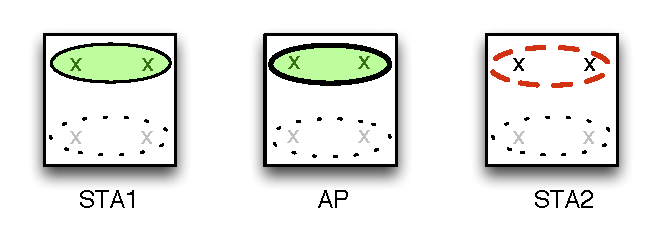
\includegraphics[width=0.5\textwidth]{images/macfilter.pdf}
		\caption{MAC filter setup} 
		\label{fig:macfilter} 
	\end{center}
\end{figure}

\begin{exercise}{Network hiding}

A first step in preventing someone to use your wireless network is to hide it from being detected by a regular scan. Hiding a \ac{ssid} ensures it will not show up in the list of available \acp{ap} when a scan is performed. You will however show that the clever sniffer is still able to detect the network.

\begin{enumerate}
	\item Set up your network as illustrated in figure \ref{fig:macfilter}, but do not set up the \ac{wnic} of \ac{sta}1 yet. \label{ex:ssidHiding1}
	\item Start a trace on the monitor interface (\file{\acs{sta}2.pcap}) of \ac{sta}2. While the trace is running, bring up the \ac{wnic} from \ac{sta}1. \label{ex:ssidHiding2} Make sure the station is associated with the \ac{ap} before you stop your trace.
	\item Indicate in which frames the \ac{ssid} is visible. Give a packet ID of an example packet in your trace file for each.\newline
	\begin{esolution}
	\end{esolution} 
	\item The next step is to hide the \ac{ssid}. This can be done adding the following line to the hostapd.conf file: \incommand{ignore\_broadcast\_ssid=1}. Bring the interface down on \ac{sta}1, restart \incommand{hostapd} on the \ac{ap} and repeat steps \ref{ex:ssidHiding1} and \ref{ex:ssidHiding2}. Save your trace to \file{STA2.pcap}.
	\item Compare the two trace files and indicate how the \ac{ssid} is hidden. In what way can a \ac{ssid} still be detected?\newline
	\begin{esolution}
	\end{esolution}
\end{enumerate}

\end{exercise}

\begin{exercise}{\ac{mac} filtering}

Continuing from the setup you used in the previous exercise, a possible intruder has still complete access to our network. In the next step, you will prevent him from joining the network by \ac{mac} filtering. 


\begin{enumerate}
	\item The management of the \ac{mac} filtering is also performed by modifying the \incommand{hostapd.conf} file at the \ac{ap}.  The entries needed for \ac{mac} filtering are:
	\begin{description}
		\item[macaddr\_acl=] controls the behaviour of the mac filtering  and expects an integer value from the following list:
		\begin{description}
			\item[0] accept unless in deny list,
			\item[1] deny unless in accept list,
			\item[2] use external RADIUS server (accept/deny lists are searched first
		\end{description}
		\item[accept\_mac\_file=] append the name of the file here that contains the list of \ac{mac} addresses to accept.
		\item[deny\_mac\_file=] append the name of the file here that contains the list of \ac{mac} addresses to deny.
	\end{description} 
	\item Configure the \ac{ap} in such a way that the \ac{mac} address of the \texttt{wlan0} interface of \ac{sta}1 is blocked from the network. SSID broadcasting may be enabled again.
	\item Now bring down the \ac{wnic} at \ac{sta}1 again, restart a capture session on \ac{sta}2 and save it to \file{\acs{sta}2.pcap}\\ and bring the \ac{wnic} back up at \ac{sta}1 when this capture session is active. Compare the results from this capture file with the first one you made and discuss the differences between both. Illustrate with packet IDs.\newline
	\begin{esolution}
	\end{esolution}
	\item Of course, in a real world setup, blocking unwanted MAC addresses is not feasible. One would use the option with the \texttt{accept\_mac\_file} parameter, allowing only known \ac{mac} addresses to connect. How would you circumvent this security measure? If an attacker has joined the network, will this have an effect on legitimate stations on that network?\newline
	\begin{esolution}
	\end{esolution}
\end{enumerate}

	
\end{exercise}




\section{Encryption}
\subsection{\acs{wep}}

The security techniques from the previous section will ``prevent'' a possible attacker from joining the network by hiding the network or preventing him access to the network. However, it is still possible to read any communication over the network by using a \ac{wnic} in monitor mode. Encryption mechanisms will counter this and obfuscate the network traffic for an eavesdropper. You will take a look at \ac{wep} here as this method is still sometimes being used although it is very vulnerable to attacks. \ac{wpa}2 is far more resilient.

\begin{exercise}{\ac{wep} encryption}
\label{ex:wep}

	\ac{wep} was the first available encryption method, standardised together with the \wifi standard. It was however quickly been proven insecure. In fact, as of 2004, \ac{wep} was declared deprecated by IEEE because of its flaws. In this exercise, you will first set up a \ac{wep} encrypted network to check what is exactly encrypted. In the next exercise you will crack the encryption key.
	
Because \ac{wep} is quite old, the tools you will use assume that IPv4 is used, as they will use \ac{arp} messages. Therefore, for this exercise, you will configure IPv4 addresses instead of IPv6 addresses.

\begin{figure}[h!]
		\begin{center}
			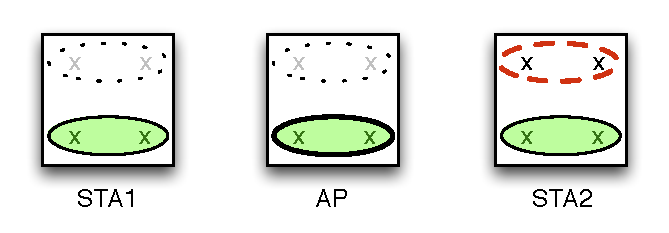
\includegraphics[width=0.5\textwidth]{images/wepcrack.pdf}
			\caption{WEP setup} 
			\label{fig:wepcrack} 
		\end{center}
	\end{figure}
	
	\begin{enumerate}
		\item Start from the network setup as shown in figure \ref{fig:wepcrack}. Disable any \ac{mac} filter that is still in place.
		\item In order to avoid capturing needless IPv4 traffic, disable the \texttt{avahi-daemon} on all three nodes:\newline
		\command{\prompt{\acs{wmn}} killall avahi-daemon}
		\item Create a tracefile on the monitor interface of \ac{sta}2 (\file{\ac{sta}2.cap}\\), containing the scan, authentication and association phase of \ac{sta}1 and a 5 packet ping session between \ac{sta}1 and \ac{sta}2. Use \texttt{10.0.\acs{gid}.1/24} for \ac{sta}1 and \texttt{10.0.\acs{gid}.2/24} for \ac{sta}2.\newline
		\command{\prompt{\acs{sta}} ip addr add 10.0.\acs{gid}.X/24 broadcast 10.0.\acs{gid}.255 dev wlan1}
		\item Make sure that \ac{sta}2 is connected to the \ac{ap} and that the \ac{wnic} of \ac{sta}1 is down before the start of the capture session. To ping, use \incommand{ping} instead of \incommand{ping6}. This trace will be our reference trace. \label{wep1} 
		\item Activate the \ac{wep} encryption on the \ac{ap}. You can choose a random key as long as it is either 5 or 13 characters long ("arandomwepkey" in this example):\newline
		Change the \incommand{hostapd.conf} file, so that it includes the following lines:\newline
		\command{wep\_key0="arandomwepkey"}
		\command{wep\_default\_key=0}
		\remark The WEP key must be \stress{exactly 5 or 13} characters long!
		\item Make sure the \ac{ap} is running. Connect \ac{sta}2 to the \ac{ap}:\newline
		\command{\prompt{\acs{sta}2} iw dev wlan1 connect wmn-0-A key 0:arandomwepkey}
		\item Make sure the interface of \ac{sta}1 is down and then start a new trace on the monitor interface of \ac{sta}2. Save it to \file{\acs{sta}2.wep.pcap}\\.
		\item Perform the same test as in step \ref{wep1}, but be sure to add \texttt{key 0:arandomwepkey} when you connect \ac{sta}1 to the network.
		\item Compare both trace files. In the second trace file, you should no longer be able to see the \incommand{ping} session in the clear.
		\begin{itemize}
			\item Which frame types are encrypted?\newline
			\begin{esolution}
			\end{esolution}
			\item Which part of a frame is encrypted and which part is still readable?\newline
			\begin{esolution}
			\end{esolution}
		\end{itemize} 
		Refer to specific frames from the second trace file to illustrate your answers.
		
	\end{enumerate}
	
\end{exercise}
	
	
	
\begin{exercise}{Cracking the \ac{wep} keys}	

	Without going into details about the flaws in  \ac{wep}, the main problem arises from the fact that traffic keys are easily repeated on a busy network. A traffic key is the key actually used by the encryption algorithm RC4.  As RC4 is a stream cipher, the same key should not be used twice. Therefore, the shared \ac{wep} key, which is configured in each \ac{ap} and \ac{sta}, is combined with a random \ac{iv}. This \ac{iv} is transmitted in plaintext between two wireless clients so the receiver can recreate the encryption key used for a specific packet, by combining the chosen (shared) network key with the received \ac{iv}. As the \ac{iv} has a length of only 3 bytes, the number of possibilities is relatively low and in busy networks, the same \acp{iv} are frequently reused, weakening the cryptographic strength of \ac{wep}. Furthermore, statistical relations between used keys and encrypted text can be exploited to find the used key.
	
	Various methods have been developed to crack a \ac{wep} key, but you will just illustrate the mere ease with which a \ac{wep} encrypted network can be hacked using the aircrack tool \cite{aircrackNG}. This tool implements various approaches, but you will limit ourselves to \ac{ptw} method. The attack is based on the fact that the first 16 bytes of an \ac{arp} packet are fixed. This is also the reason we switched to IPv4 for this exercise\ldots For more details read \cite{cryptoeprint:2007:120}, specifically sections 1 and 5 for a general overview. Exploiting the relation between cleartext and the captured \acp{iv} makes it possible to quite easily determine the network key.
	
	\begin{figure}[h!]
		\begin{center}
			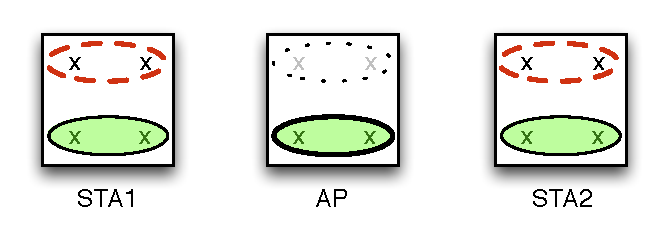
\includegraphics[width=0.5\textwidth]{images/wepcrack2.pdf}
			\caption{WEP cracking setup} 
			\label{fig:wepcrack2} 
		\end{center}
	\end{figure}
	
	
	\begin{enumerate}
		\item Before you start to crack the configured \ac{wep} key, first have a second look at the traces from the previous exercise. Using Wireshark\cite{wireshark}, you can decrypt an encrypted trace. Using the menu Edit$\rightarrow$ Preferences $\rightarrow$ Protocols $\rightarrow$ IEEE 802.11 you can specify the key in HEX. To convert your key to HEX, use e.g. the following website: \url{http://www.dirtymonday.net/key_convert.html} For our example it will be \incommand{6172616E646F6D7765706B6579}.\newline
Make sure you also check the `decrypt packets' box. Select an ICMP request in both trace files (unencrypted and encrypted, but decrypted by Wireshark) and identify the extra information added to a frame in order to encrypt it. Also indicate where in the frame this information is added.\newline
		\begin{esolution}
		\end{esolution}
		\item Start from the \ac{wep} encrypted network you created in the previous exercise.
		\item Add an additional monitor interface on \ac{sta}1, resulting in the network scheme shown in figure \ref{fig:wepcrack2}. The monitor interface on \ac{sta}2 will be used to perform the actual attack. \ac{arp} packets will be injected into the network in order to trigger \ac{arp} responses which will contain new \acp{iv} with every response . These packets will be captured and stored in files. In parallel with this capturing of new \ac{arp} responses and the associated \acp{iv}, we can start the process of analyzing these packages and searching for the key. The monitor interface on \ac{sta}1 will be used to monitor the channel so we can afterwards take a look at what happened.
		\item Start a packet capture to \file{\acs{sta}1.pcap}\\ on the monitor interface of \ac{sta}1.
		\item Start the \ac{iv} capture process at \ac{sta}2. This command will store its captured frames in files \incommand{output-xy.cap} and \incommand{output-xy.txt}. Make sure to run this command with your active directory set to the \texttt{/mnt} folder, in which a remote directory is mounted.\newline
		\command{\prompt{STA2} airodump-ng --band a --channel x --bssid <\acs{mac} addr \acs{ap}> -w output wlan0}
		This should give you an overview screen where at least the incoming beacon count is rising. If no activity is shown, bring the interface down and then bring it up again and retry. This command will store its captured frames in files \incommand{output-xy.cap} and \incommand{output-xy.txt}. Make sure to run this command in \texttt{/mnt}, where a remote location is mounted.\newline
		\item On a new terminal, perform a fake authentication to the \ac{ap} from the attacking machine (\ac{sta}2). This ensures the frames we will be injecting for \texttt{wlan1} will be accepted by the \ac{ap}:\newline
		\command{\prompt{STA2} aireplay-ng --fakeauth 0 -e wmn-\acs{gid}-A -a <\acs{mac} addr \acs{ap}> -h <\acs{mac} addr wlan0> wlan0.}	
		\item It is now time to actively inject packets into the wireless network. This is done by the following command:
		 \command{\prompt{STA2} aireplay-ng --arpreplay -b <MAC addr AP> -h <MAC addr wlan0> -x 1024 -o 512 wlan0}\newline
		 This command will monitor incoming packets and when an \ac{arp} request passes, it will re-inject it at a rate of several 100 frames/s.  You should be able to see this in the output from \incommand{airodump-ng}.\newline
		 \remark Due to a bug in the driver, the packet injection rate will not be high enough. You should run 10 of the above \incommand{aireplay-ng} commands in parallel to generate enough packets. You can do so easily by editing the \texttt{wepcrack.sh} script found on the nodes. Insert the correct \ac{mac} addresses in that script and run it. To stop the replay attack, simply type \incommand{killall aireplay-ng}.
		  \item In order to get an \ac{arp} request, just start a ping from \ac{sta}1 to \ac{ap}. This should trigger an \ac{arp} request. If the \ac{arp} tables already contained the IP addresses from both hosts (check it with \incommand{\prompt{STA1} ip neigh}), remove the entry using \incommand{ip neigh flush dev wlan1}.
		 \item To crack the key, the tool \incommand{aircrack-ng} can be used. This tool processes the files generated by \incommand{airodump-ng}. The needed number of packets to crack the key depends on the bit length of the key. In general, you need at least 20,000 packets for a 64-bit key and between 40,000 and 85,000 for a 128-bit key. To start the analysis, run the following command in the folder containing the output from \incommand{airodump-ng}:\newline
		\command{\prompt{STA2} aircrack-ng -b  <\acs{mac} addr \acs{ap}> output*.cap -q}
		\item If you captured enough packets, after a while, the \incommand{aircrack-ng} tool should provide you with the \ac{wep} key used in your network. Copy its output here:\newline
		\begin{esolution}
		\end{esolution}
		\item Using the following \incommand{tshark} command on a lab PC, you can get a list of \acp{iv} used during your session. \newline
		\command{tshark -r <trace file> -T fields -e wlan.wep.iv}
		\item How many \acp{iv} did you capture? And how many of them occured at least twice?\newline
		\begin{esolution}
		\end{esolution}	
	\item When handing in the report, you must include the \texttt{output-*.csv} and \texttt{*.netxml} files. \texttt{output-*.cap} is not required, as it will be quite large. Limit the trace file of \ac{sta}1 to only a few (e.g. a hundred) of packets that show the \ac{arp} injection in progress.
	\end{enumerate} 
		
\end{exercise}

\subsection{\acs{wpa}2}

As you have demonstrated in the previous exercise, \ac{wep} encryption is easily circumvented. You will now take a look at \ac{wpa}2 encryption. You will no try to crack it, as \ac{wpa}2 uses the \ac{ccmp} algorithm with \ac{aes} encryption, which is extremely resilient to attacks. To give you an idea, the best known method until now to crack a 128 bit \ac{aes} key, which is used by \ac{wpa}2, still takes at least \( 2^{126.1} \) computations\cite{cryptoeprint:2011:449}.

A security flaw concerning \ac{wps} has been discovered that makes \acp{ap} running \ac{wps} vulnerable to a relatively easy attack (which would still take far too much time for this lab exercise)\cite{wps}. This, of course, does not hold true for \acp{ap} that do not have \ac{wps} enabled. If you want to read up on how \ac{wpa}2 works and on the evolution in security from \ac{wep} over \ac{wpa} to \ac{wpa}2, you should read \cite{wifisecurity:2012}.

\begin{exercise}{\acs{wpa}2}

\begin{figure}[h!]
		\begin{center}
			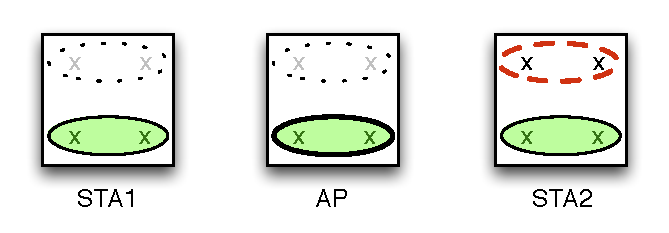
\includegraphics[width=0.5\textwidth]{images/wepcrack.pdf}
			\caption{\acs{wpa} setup} 
			\label{fig:wpa} 
		\end{center}
	\end{figure}

\begin{enumerate}
	\item Start from the \ac{wpa}2 enabled network setup as seen in figure \ref{fig:wpa}.
	\item On the \ac{ap}, to enable \ac{wpa}2, make sure that the line \texttt{wpa=0} in the \texttt{hostapd.conf} file is changed to \texttt{wpa=2}, and add the following lines to \texttt{hostapd.conf}:
	\begin{verbatim}
		wpa_passphrase=aRandomPassphrase
		wpa_key_mgmt=WPA-PSK
		rsn_pairwise=CCMP
	\end{verbatim}
	\remark Use your own passphrase if you like. Unlike \ac{wep}, it is not restricted to a certain amount of characters.
	\item Set the IP addresses of \texttt{wlan1} on \ac{sta}1 and \ac{sta}2 to \texttt{fc00:\acs{gid}::1/64} and \texttt{fc00:\acs{gid}::2/64}, respectively.
	\item Connect \ac{sta}2 to the network. In order to do so, modify the \texttt{wpa\_supplicant.conf} file so that it includes the correct \acs{essid} and passhprase. Afterwards, run:\newline
	\command{\prompt{\acs{sta}2} wpa\_supplicant -B -c/root/wpa\_supplicant.conf -iwlan1}
	\remark You might get an error like \texttt{ioctl[SIOCSIWENCODEEXT]: Invalid argument}. You can safely ignore this error.
	\item Make sure the monitor interface on \ac{sta}2 is configured and start a trace. Save it in \file{\acs{sta}2.pcap}\\.
	\item Now bring the interface on \ac{sta}1 up an do \texttt{ping6 -c 5} to \ac{sta}2.
	\item Which frame types are encrypted? Give examples.\newline
		\begin{esolution}
		\end{esolution}
	\item Which part of a frame is encrypted and which part is still readable?\newline
		\begin{esolution}
		\end{esolution}
		\item Compare this trace file with the one made in exercise \ref{ex:wep}. Compare the authentication/association phase of \ac{sta}1. What are the similarities and what are the differences? Refer to packet IDs!\newline
		\begin{esolution}
		\end{esolution}
		\item Now, compare an encrypted frame in both traces. Indicate where they differ.\newline
		\begin{esolution}
		\end{esolution}
\end{enumerate}

\end{exercise}



\section{Denial of Service Attacks}

\begin{figure}[h!]
		\begin{center}
			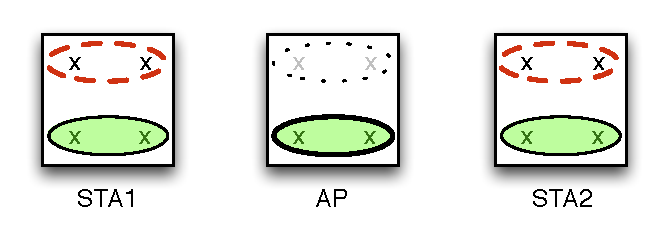
\includegraphics[width=0.5\textwidth]{images/wepcrack2.pdf}
			\caption{DoS setup} 
			\label{fig:dos} 
		\end{center}
	\end{figure}

In the previous section, you have gained access to a \ac{wep} encrypted network by actively injecting packets and cracking the key. This kind of attack makes it possible that you, the attacker, can afterwards associate with the network and sniff all traffic on that network. Alternatively, you can also use the network yourself as if you were a normal user.

Within this section, you will illustrate a \ac{dos} attack that shows the vulnerability of a wireless network. You will not gain access to the network as such, but you will disturb normal network operation. Tools to do so are freely available and current encryption techniques cannot prevent these attacks as they make use of management frame injection. As you have seen, management frames are not encrypted and thus can be easily injected into a wireless network. 

\begin{exercise}{Disassociation Attack}
	
	The principle behind a disassociation attack is quite easy. A disassociation frame is sent by either a \ac{sta} or \ac{ap} to signal the disconnection from the wireless network. For instance, it is sent by a \ac{sta} just before you disable an associated \ac{wnic}. Although the sending of a disassociation message is not mandatory by the standard, at reception of such frame, a client should consider its connection lost and an \ac{ap} will remove a \ac{sta} from the list of connected stations. Injecting a malicious disassociation frame for a wireless node will thus force this node to scan for and associate again to its \ac{ap}, resulting in a connectionless period. If the disassociation frame is sent periodically, this can render the wireless network useless to the attacked \ac{sta}.

\begin{enumerate}
	\item Start from the network scheme as illustrated in figure \ref{fig:dos}.
	\item Be sure to have configured your network with \ac{wpa}2 encryption.
	\item Configure the IP addresses of \ac{sta}1 and \ac{sta}2  to \texttt{fc00:\acs{gid}::1/64} and\newline \texttt{fc00:\acs{gid}::2/64} respectively.
	\item On the monitor interface of \ac{sta}1, start a capture session and save it to\newline \file{\acs{sta}1.pcap}\\.
	\item Start a \incommand{ping6} from \ac{sta}1 to \ac{sta}2.
	\item On \ac{sta}2, use the following command to send a disassociation to \ac{sta}1:\newline
	\command{\prompt{STA2}  aireplay-ng --deauth 1 wlan0 -a <MAC addr AP> -c <MAC addr STA1>}
	\item What is the result for the ping?\newline
	\begin{esolution}
	\end{esolution}
	\item Open the trace file and explain using this trace what exactly happened.\newline
	\begin{esolution}
	\end{esolution}

\end{enumerate} 	
	
\end{exercise}

%\backmatter

\chapter*{Acronyms} 
\addcontentsline{toc}{chapter}{Acronyms} 
\markboth{Acronyms}{Acronyms} 
%!TEX root =labo.tex

\begin{acronym}
\acro{aes}[AES]{Advanced Encryption Standard}
\acro{ap}[AP]{access point}
\acro{arp}[ARP]{Address Resolution Protocol}
\acro{bipt}[BIPT]{Belgisch Instituut voor Postdiensten en Telecommunicatie - Belgian Institute for Postal services and Telecommunications}
\acro{bss}[BSS]{basic service set}
\acro{bssid}[BSSID]{\acl{bss} ID}
\acro{ccmp}[CCMP]{Counter Cipher Mode with Block Chaining Message Authentication Code Protocol}
\acro{cts}[CTS]{Clear to Send}
\acro{dhcp}[DHCP]{Dynamic Host Configuration Protocol}
\acro{dos}[DoS]{denial of service}
\acro{essid}[ESSID]{extended \acl{ssid}}
\acro{gid}[grID]{group ID}
\acro{ibss}[IBSS]{independent \acl{bss}}
\acro{icmp}[ICMP]{Internet Control Message Protocol}
\acro{iv}[IV]{initialization vector}
\acro{mimo}[MIMO]{multiple-input, multiple-output}
\acro{mac}[MAC]{Media Access Control}
\acro{mtu}[MTU]{Maximum Transferable Unit}
\acro{nat}[NAT]{Network Address Translation}
\acro{nd}[ND]{Neighbor Discovery}
\acro{nic}{network interface card}
\acro{ptw}[PTW]{Pychkine, Tews, Weinmann}
\acro{pxe}[PXE]{preboot execution environment}
\acro{ram}[RAM]{Random Access Memory}
\acro{rts}[RTS]{Request to Send}
\acro{rtt}[RTT]{round trip time}
\acro{ssh}[SSH]{secure shell}
\acro{ssid}[SSID]{Service Set ID}
\acro{sta}[STA]{station}
\acro{tcp}[TCP]{Transmission Control Protocol}
\acro{udp}[UDP]{User Datagram Protocol}
\acro{vap}[VAP]{virtual access point}
\acro{wan}[WAN]{wide area network}
\acro{wep}[WEP]{Wired Equivalent Privacy}
\acro{wmn}{wireless mesh node}
\acro{wnic}{wireless \acl{nic}}
\acro{wpa}[WPA]{Wi-Fi Protected Access}
\acro{wps}[WPS]{Wi-Fi Protected Setup}
\end{acronym}


%\chapter*{Bibliography}
\bibliographystyle{plainurl}
\bibliography{wmn}

\end{document}
 
